\documentclass{article}

\usepackage{graphicx}
\usepackage[utf8]{inputenc}
\usepackage[T5]{fontenc}
\usepackage[fontsizes=14pt]{scrextend}
\usepackage[paperheight=29.7cm,paperwidth=21cm,right=2cm,left=3cm,top=2cm,bottom=2cm]{geometry}
\usepackage{mathptmx}
\usepackage{float}
\usepackage{tikz}
\usepackage{eso-pic}
\usetikzlibrary{calc}
\usepackage{fontawesome}
\usepackage{setspace}
\usepackage{titlesec}
\usepackage{indentfirst}
\usepackage{ragged2e}
\usepackage{array}
\usepackage{tocloft}
\usepackage{enumitem}
%\usepackage{tocbibind}
\usepackage[hidelinks]{hyperref}
\usepackage{etoolbox}
\counterwithin{figure}{section} % đánh số hình theo section
\renewcommand{\figurename}{Hình} % đổi Figure -> Hình
\usepackage{cite}              % trích dẫn IEEE
\usepackage{hyperref}  % cải thiện hiển thị URL
\usepackage{listings}
\usepackage{xcolor}
\usepackage{hyphenat}


% --- xử lý URL dài: cho phép xuống dòng trong link ---
\usepackage[hidelinks]{hyperref}
\usepackage{xurl}           % cho phép ngắt ở hầu hết vị trí trong URL

\usepackage{caption}

\hyphenation{} % bỏ tách chữ


% Tạo font mới tên là my14pt nghiêng
\DeclareCaptionFont{my14pt}{\fontsize{14pt}{16pt}\selectfont\itshape} % Áp dụng cho caption của figure 
\captionsetup[figure]{ 
    labelformat=simple, 
    labelsep=colon, 
    justification=centering,  
    font=my14pt 
}


% Cấm orphan / widow để dùng cho toàn tài liệu (không trong \setlist):
\clubpenalty=10000
\widowpenalty=10000
\displaywidowpenalty=10000

% --- Định dạng section (CHƯƠNG) ---
\let\oldsection\section
\renewcommand{\section}[1]{%
  \refstepcounter{section}%
  \addcontentsline{toc}{section}{CHƯƠNG \thesection: #1}%
  \par\vspace{3pt}% khoảng cách phía trên
  {\setstretch{1.5}%
    \noindent\centering\bfseries\fontsize{14pt}{18pt}\selectfont
    CHƯƠNG \thesection: #1\par}%
  \vspace{3pt}% khoảng cách phía dưới
}

% --- Định dạng section* (không số) ---
\newcommand{\sectionstar}[1]{%
  \par\vspace{3pt}% khoảng cách phía trên
  {\setstretch{1.5}%
    \noindent\centering\bfseries\fontsize{14pt}{18pt}\selectfont
    #1\par}%
  \vspace{3pt}% khoảng cách phía dưới
  \addcontentsline{toc}{section}{#1}%
}


%\titlespacing*{\section}{0pt}{3pt}{3pt}

% --- Định dạng subsection ---
\titleformat{\subsection}[block]
  {\parindent=1cm\noindent\hspace*{1cm}\bfseries\fontsize{14pt}{18pt}}
  {\thesubsection.}
  {1em}
  {}

\titleformat{name=\subsection,numberless}[block]
  {\centering\bfseries\fontsize{14pt}{18pt}}
  {}
  {0em}
  {}

\titlespacing*{\subsection}{0pt}{3pt}{3pt}


\lstset{
    language=Python,
    basicstyle=\ttfamily\large,
    keywordstyle=\color{blue},
    stringstyle=\color{red},
    commentstyle=\color{green},
    numbers=none,       % tắt số dòng
    stepnumber=1,
    numbersep=5pt,
    xleftmargin=0pt,
    frame=single,
    breaklines=true,
    showstringspaces=false
}


\newlist{myitem}{itemize}{1}
\setlist[myitem,1]{%
  label=--,           % dấu gạch ngang
  labelindent=1cm,    % dòng đầu tiên thụt 1cm
  labelsep=0.5cm,     % khoảng cách từ dấu - đến chữ đầu
  leftmargin=0pt,      % lề tổng = 0, dòng sau căn sát lề văn bản
  align=left,          % dòng tiếp theo căn trái
  labelwidth=*,       
  itemsep=6pt,        % khoảng cách giữa các item
  topsep=6pt           % khoảng cách giữa danh sách và đoạn ngoài
}

\newlist{mysubitem}{itemize}{1}
\setlist[mysubitem,1]{%
  label=\textbf{+},      % dấu +
  labelindent=1.5cm,     % thụt lề nhãn
  labelsep=0.5cm,        % khoảng cách nhãn - nội dung
  leftmargin=0cm,        % tổng thụt lề (labelindent + labelwidth + labelsep)
  align=left,          % dòng tiếp theo căn trái
  labelwidth=*,       
  align=parleft,         % căn lề cho dòng thứ 2
  itemsep=6pt,           % khoảng cách giữa các item
  topsep=6pt             % khoảng cách trước/sau list
}

\titleformat{\subsubsection}[block]
  {\parindent=1cm\noindent\hspace*{1cm}\bfseries\itshape\fontsize{13pt}{17pt}}
  {\thesubsubsection.}
  {1em}
  {}

\titlespacing*{\subsubsection}{0pt}{3pt}{3pt}

% --- Định dạng mục lục ---


% --- Định dạng nội dung chính ---
\newenvironment{maincontent}{
  \onehalfspacing
  \setlength{\parindent}{1cm}
  \setlength{\parskip}{6pt}
  \fontsize{14pt}{21pt}\selectfont
  
  % Ngăn orphan / widow
  \clubpenalty=10000          % cấm dòng đầu bị rớt xuống cuối trang
  \widowpenalty=10000         % cấm dòng cuối bị đẩy sang trang mới
  \displaywidowpenalty=10000  % cấm widow trước công thức
}{}


% --- Môi trường cho trang tiêu đề ---
\newenvironment{titlepaper}{\thispagestyle{empty}}{}

\newcommand{\plainsection}[1]{%
  \par\vspace{6pt}% khoảng cách phía trên
  \phantomsection
  {\setstretch{1.5}%
  \noindent\centering\bfseries\fontsize{14pt}{18pt}\selectfont #1\par}%
  \vspace{6pt}% khoảng cách phía dưới
}



\begin{document}

% Tạo lệnh \subsubsubsection
\newcounter{subsubsubsection}[subsubsection]
\renewcommand{\thesubsubsubsection}{\thesubsubsection.\arabic{subsubsubsection}}

\newcommand{\subsubsubsection}[1]{%
  \refstepcounter{subsubsubsection}%
  \par\vspace{6pt}%
  {\parindent=1cm
   \noindent\hspace*{1cm}\itshape\fontsize{14pt}{18pt}\selectfont
   \thesubsubsubsection.\quad #1\par}%
  \vspace{3pt}%
}

\thispagestyle{empty}
% Trang bìa
\begin{titlepaper}
\begin{tikzpicture} [overlay,remember picture]
\draw [line width=3pt]
    ($ (current page.north west) + (3.0cm,-2.0cm) $)
    rectangle
    ($ (current page.south east) + (-2.0cm,2.5cm) $);
\draw [line width=0.5pt]
    ($ (current page.north west) + (3.1cm,-2.1cm) $)
    rectangle
    ($ (current page.south east) + (-2.1cm,2.6cm) $);
\end{tikzpicture}

\begin{center}
\vspace{-6pt} \textbf{\fontsize{14pt}{18pt}\selectfont HỌC VIỆN AN NINH NHÂN DÂN}\\
\textbf{\fontsize{14pt}{18pt}\selectfont KHOA ANM VÀ PCTPSDCNC}\\
\textbf{\fontsize{14pt}{18pt}\selectfont -------------}\\[2.0cm]


\includegraphics[width = 0.27\textwidth]{img/Logo_hoc_vien_ANND.png}\\[1.5cm]

\textbf{\fontsize{20pt}{18pt}\selectfont BÀI TIỂU LUẬN}\\[1.0cm]
\begin{minipage}{\dimexpr\paperwidth - 6cm} % 3cm + 1cm bên trái và 2cm + 1cm bên phải
\centering
\textbf{\fontsize{22pt}{18pt}\selectfont AN TOÀN ĐIỆN TOÁN ĐÁM MÂY VÀ XỬ LÝ DỮ LIỆU LỚN}\\[2.0cm]
\end{minipage}\\[1.0cm]


\renewcommand{\baselinestretch}{1.75}\normalsize
\begin{spacing}{2.0}
\begin{minipage}{\dimexpr\paperwidth - 6cm} % 3cm + 1cm bên trái và 2cm + 1cm bên phải
\centering
\textbf{\fontsize{14pt}{18pt}\selectfont TÊN ĐỀ TÀI: TÌM HIỂU VÀ KHAI THÁC DỊCH VỤ ĐÁM MÂY CỦA ORACLE CLOUD}
\end{minipage}\\[1.0cm]
\end{spacing}

\begin{tikzpicture}[remember picture, overlay]
    \node[anchor=north] at ($ (current page.south west) + (3.5cm,3.5cm) + (7.8cm,0) $)
        {\fontsize{14pt}{18pt}\selectfont Hà Nội, \ifnum\month<10 0\number\month\else\number\month\fi/\number\year};
\end{tikzpicture}

\end{center}
\end{titlepaper}

\newpage

%\begin{titlepaper}
\begin{tikzpicture} [overlay,remember picture]
\draw [line width=3pt]
    ($ (current page.north west) + (3.0cm,-2.0cm) $)
    rectangle
    ($ (current page.south east) + (-2.0cm,2.5cm) $);
\draw [line width=0.5pt]
    ($ (current page.north west) + (3.1cm,-2.1cm) $)
    rectangle
    ($ (current page.south east) + (-2.1cm,2.6cm) $);
\end{tikzpicture}

\begin{center}
\vspace{-6pt} 
\textbf{\fontsize{14pt}{18pt}\selectfont HỌC VIỆN AN NINH NHÂN DÂN}\\
\textbf{\fontsize{14pt}{18pt}\selectfont KHOA ANM VÀ PCTPSDCNC}\\
\textbf{\fontsize{14pt}{18pt}\selectfont -------------}\\[1.5cm]


\includegraphics[width = 0.24\textwidth]{img/Logo_hoc_vien_ANND.png}\\[1.0cm]

\textbf{\fontsize{20pt}{18pt}\selectfont BÀI TẬP LỚN}\\[1.0cm]
\textbf{\fontsize{25pt}{18pt}\selectfont THÂM NHẬP GIẢ ĐỊNH}\\[1.5cm]

\renewcommand{\baselinestretch}{1.75}\normalsize
\begin{spacing}{2.0}
\begin{minipage}{\dimexpr\paperwidth - 6cm} % 3cm + 1cm bên trái và 2cm + 1cm bên phải
\centering
\textbf{\fontsize{14pt}{18pt}\selectfont TÊN ĐỀ TÀI: THỰC NGHIỆM MỘT SỐ KỊCH BẢN THÂM NHẬP GIẢ ĐỊNH}
\end{minipage}\\[1.0cm]
\end{spacing}

% ==== Thêm thông tin trình bày ====
\vspace{1.4cm} % Khoảng cách dưới tên đề tài

{\fontsize{14pt}{14pt}\selectfont
\begin{center}
\vspace{-6pt} 
\begin{tabular}{ l l }
\textbf{Giảng viên hướng dẫn} & : Đại úy Nguyễn Trọng Hưng \\
\textbf{Nhóm trình bày}  & : Nhóm 2 \\
\textbf{Trung đội}            & : B14D52 \\
\end{tabular}
\end{center}
}


\begin{tikzpicture}[remember picture, overlay]
    \node[anchor=north] at ($ (current page.south west) + (3.5cm,3.5cm) + (7.8cm,0) $)
        {\fontsize{14pt}{18pt}\selectfont Hà Nội, \ifnum\month<10 0\number\month\else\number\month\fi/\number\year};
\end{tikzpicture}

\end{center}
\end{titlepaper}

%\thispagestyle{empty}
%\newpage

\thispagestyle{empty}
\input{sophach}
\newpage

% Nội dung chính
\begin{maincontent}

\clearpage
\begingroup
  \makeatletter
  \let\ps@plain\ps@empty   % ép plain = empty
  \pagestyle{empty}
  \plainsection{MỤC LỤC}
\renewcommand{\contentsname}{}  % Xoá tiêu đề mặc định
\renewcommand{\cftsecleader}{\cftdotfill{\cftdotsep}}
\renewcommand{\cftsecfont}{\normalfont}
\renewcommand{\cftsecpagefont}{\normalfont}

% -- In đậm cho section (CHƯƠNG) và subsection --
\renewcommand{\cftsecfont}{\bfseries}        % tên section in đậm
\renewcommand{\cftsecpagefont}{\bfseries}    % số trang section in đậm
\renewcommand{\cftsubsecfont}{\bfseries}     
\renewcommand{\cftsubsecpagefont}{\bfseries} 
\renewcommand{\cftsubsubsecfont}{\normalfont}     
\renewcommand{\cftsubsubsecpagefont}{\normalfont}

% --- Giãn dòng và khoảng cách ---
\renewcommand{\baselinestretch}{1.15}\selectfont  % line spacing 1.15

% khoảng cách trên dưới mỗi mục (section, subsection...)
\setlength{\cftbeforesecskip}{6pt}
\setlength{\cftbeforesubsecskip}{6pt}
\setlength{\cftbeforesubsubsecskip}{6pt}

\thispagestyle{empty}
\tableofcontents

  \clearpage
  \begingroup

  \renewcommand{\listfigurename}{DANH MỤC HÌNH ẢNH}

  % --- Định dạng tiêu đề ---
  \renewcommand{\cftloftitlefont}{\hfill\fontsize{14pt}{21pt}\selectfont\bfseries}
  \renewcommand{\cftafterloftitle}{\hfill}

  % --- Tiền tố "Hình" trước số hình ---
  \renewcommand{\cftfigpresnum}{Hình~}
  \renewcommand{\cftfigaftersnum}{:~}

  % --- Khoảng cách tự động từ số hình đến nội dung ---
  \cftsetindents{figure}{0pt}{4.5em}  
  % 0pt = sát lề trái
  % 2em = khoảng cách từ "Hình x:" đến nội dung, LaTeX tự dãn nếu số dài

  % --- Định dạng dòng danh mục ---
  \renewcommand{\cftfigfont}{\fontsize{14pt}{21pt}\selectfont}
  \renewcommand{\cftfigpagefont}{\fontsize{14pt}{21pt}\selectfont}

  % --- Khoảng cách giữa các dòng trong danh mục hình ảnh ---
  \setlength{\cftbeforefigskip}{6pt}

  % --- Giãn dòng 1.15 ---
  \renewcommand{\baselinestretch}{1.15}\selectfont
  \listoffigures
\endgroup

  \clearpage
\makeatother
\endgroup

% quay lại đánh số bình thường cho nội dung chính
\pagestyle{plain}

\clearpage
\pagenumbering{arabic} % Bắt đầu đánh số 1, 2,...

% Định dạng số trang
\renewcommand{\thepage}{\fontsize{14pt}{16pt}\selectfont\arabic{page}}

\setcounter{page}{1}
\plainsection{MỞ ĐẦU}
\addcontentsline{toc}{section}{MỞ ĐẦU}

\textbf{1. Lý do chọn đề tài}

Trong thời đại số, công nghệ điện toán đám mây đã trở thành nền tảng quan trọng giúp các tổ chức tối ưu hóa nguồn lực, giảm chi phí đầu tư hạ tầng và nâng cao năng lực cạnh tranh. Thay vì phải duy trì hệ thống máy chủ vật lý tốn kém, các doanh nghiệp có thể khai thác tài nguyên tính toán, lưu trữ và dịch vụ phần mềm trực tiếp trên nền tảng đám mây với mức độ linh hoạt và khả năng mở rộng gần như vô hạn.

Oracle Cloud Infrastructure (OCI) là một trong những nền tảng đám mây đang phát triển mạnh, nổi bật với thế mạnh về cơ sở dữ liệu, khả năng xử lý hiệu năng cao, đồng thời cung cấp hệ sinh thái dịch vụ đa dạng từ IaaS, PaaS đến SaaS. Ngoài ra, OCI còn chú trọng vào bảo mật, tự động hóa và hỗ trợ trí tuệ nhân tạo, đáp ứng tốt nhu cầu chuyển đổi số toàn diện.

Đối với Việt Nam, khi chương trình chuyển đổi số quốc gia đang được thúc đẩy mạnh mẽ, việc nghiên cứu và nắm bắt công nghệ Oracle Cloud là cần thiết để sinh viên, nhà nghiên cứu và doanh nghiệp có thể tiếp cận, làm chủ công nghệ, từ đó ứng dụng vào thực tế. Đây chính là lý do đề tài “Tìm hiểu và khai thác dịch vụ đám mây của Oracle Cloud” được lựa chọn.

\textbf{2. Mục tiêu nghiên cứu}

Trình bày tổng quan về điện toán đám mây và kiến trúc của Oracle Cloud Infrastructure.

Làm quen với các dịch vụ cơ bản như tính toán (Compute), lưu trữ (Object Storage, Block Storage), cơ sở dữ liệu (Autonomous Database, MySQL Database).

Tiến hành thử nghiệm triển khai, cấu hình và quản lý tài nguyên trên OCI.

Phân tích ưu điểm, hạn chế và đề xuất các hướng ứng dụng của OCI tại Việt Nam.

Hình thành kỹ năng tư duy và thực hành giải pháp trên môi trường đám mây.

\textbf{3. Phạm vi nghiên cứu}

Các dịch vụ nền tảng: IaaS (máy chủ ảo, lưu trữ, mạng), PaaS (cơ sở dữ liệu, phân tích dữ liệu), SaaS (ứng dụng doanh nghiệp).

Các công cụ triển khai và quản lý: OCI Console, Command Line Interface (CLI), Terraform.


Đối tượng nghiên cứu chủ yếu là sinh viên, nhà nghiên cứu và doanh nghiệp vừa và nhỏ có nhu cầu ứng dụng điện toán đám mây.

\textbf{4. Phương pháp nghiên cứu}

Nghiên cứu tài liệu: Thu thập và tổng hợp kiến thức từ tài liệu chính thức của Oracle, giáo trình, bài báo khoa học và các nguồn tham khảo đáng tin cậy.

Thực hành trực tiếp: Tạo tài khoản OCI, triển khai thử nghiệm máy chủ ảo, lưu trữ dữ liệu, thiết lập cơ sở dữ liệu và sử dụng một số dịch vụ AI/ML.

Đánh giá so sánh: Xem xét các yếu tố hiệu suất, chi phí, độ tin cậy và khả năng mở rộng của OCI, so với nhu cầu thực tế của các tổ chức.

\textbf{5. Bố cục đề tài}

Ngoài phần mở đầu và kết luận, bài tiểu luận được xây dựng có bố cục như sau:

\textbf{Chương 1: }Tổng quan về điện toán đám mây.

\textbf{Chương 2: }Công nghệ ảo hóa của Oracle Cloud.

\textbf{Chương 3: }Tìm hiểu và khai thác dịch vụ điện toán đám mây Oracle Cloud.

\newpage

\section{TỔNG QUAN VỀ ĐIỆN TOÁN ĐÁM MÂY}
\subsection{Khái niệm và đặc điểm của điện toán đám mây}
\subsubsection{Lịch sử ra đời của điện toán đám mây}
Khái niệm điện toán đám mây ra đời từ những năm 1950 khi máy chủ tính toán quy mô lớn (large-scale mainframe computers) được triển khai tại một số cơ sở giáo dục và tập đoàn lớn. Tài nguyên tính toán của các hệ thống máy chủ được truy cập từ các máy khách cuối (thin clients, terminal computers), từ đó khai sinh khái niệm “chia sẻ thời gian” (time-sharing) đặc tả việc cho phép nhiều người sử dụng cùng chia sẻ đồng thời một tài nguyên tính toán chung.

Trong những năm 1960 – 1990, xuất hiện luồng tư tưởng coi máy tính hay tài nguyên công nghệ thông tin có thể được tổ chức như hạ tầng dịch vụ công cộng (public utility). Điện toán đám mây hiện tại cung cấp tài nguyên tính toán dưới dạng dịch vụ và tạo cảm giác cho người dùng về một nguồn cung ứng là vô tận. Đặc tính này có thể so sánh tới các đặc tính của ngành công nghiệp tiêu dùng dịch vụ công cộng như điện và nước. Khi sử dụng điện hay nước, người dùng không cần quan tâm tới tài nguyên đến từ đâu, được xử lý, phân phối như thế nào, họ chỉ việc sử dụng dịch vụ và trả tiền cho nhà cung cấp theo lượng tiêu dùng của mình.

Những năm 1990, các công ty viễn thông từ chỗ cung ứng kênh truyền dữ liệu điểm tới điểm (point-to-point data circuits) riêng biệt đã bắt đầu cung ứng các dịch vụ mạng riêng ảo với giá thấp. Thay đổi này tạo tiền đề để các công ty viễn thông sử dụng hạ tầng băng thông mạng hiệu quả hơn. Điện toán đám mây mở rộng khái niệm chia sẻ băng thông mạng này qua việc cho phép chia sẻ cả tài nguyên máy chủ vật lý bằng việc cung cấp các máy chủ ảo.

Amazon cung cấp nền tảng Amazon Web Services (AWS) vào năm 2006, đánh dấu việc thương mại hóa điện toán đám mây. Từ đầu năm 2008, Eucalyptus được giới thiệu là nền tảng điện toán đám mây mã nguồn mở đầu tiên, tương thích với API của AWS. Tính tới thời điểm hiện tại, có rất nhiều các sản phẩm điện toán đám mây được đưa ra như Google App Engine, Microsoft Azure, Nimbus,..

\subsubsection{Khái niệm điện toán đám mây}
Điện toán đám mây là một mô hình cho phép thuận tiện, truy cập mạng theo yêu cầu đến một nơi chứa các nguồn tài nguyên tính toán có thể chia sẻ và cấu hình được (ví dụ: mạng, máy chủ, lưu trữ, ứng dụng và dịch vụ), có thể được cung cấp và phát hành nhanh chóng với nỗ lực quản lý hoặc tương tác với nhà cung cấp tối thiểu \cite{hostvn_cloud_computing}.
\begin{figure}[H] % cần gói float nếu muốn fix vị trí
    \centering
    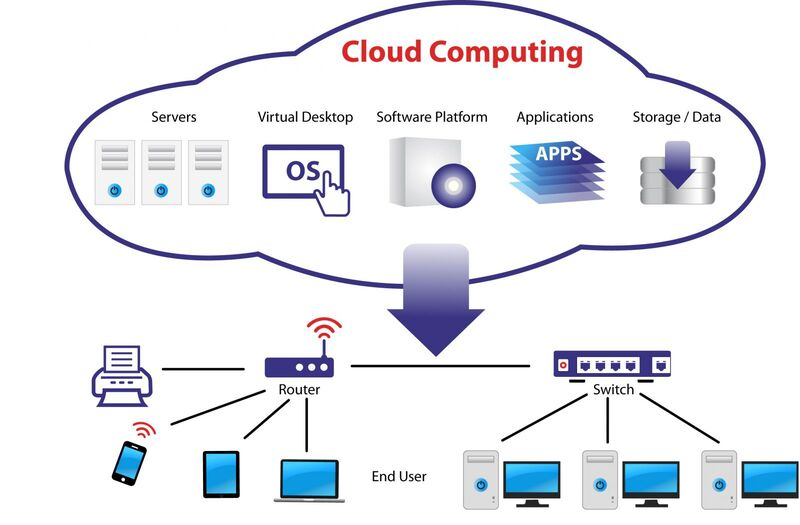
\includegraphics[width=0.7\textwidth]{Tong_quan_DTDM/dien-toan-dam-may-la-gi.jpg}
    \caption{Kiến trúc mô hình điện toán đám mây}
    \label{fig:cloud_intro}
\end{figure}

Điện toán đám mây (cloud) có thể được sử dụng cho nhiều mục đích khác nhau: machine learning, data analysis, storage \& backup, streaming media content và hơn thế nữa. Một ví dụ thực tế, tất cả các chương trình và phim bạn xem trên Netflix thực sự được lưu trữ trên đám mây. Ngoài ra, đám mây có thể có lợi cho việc tạo và thử nghiệm các ứng dụng, tự động hóa việc phân phối phần mềm và lưu trữ v.v..\cite{aws_cloud_file_storage}.

Các nhà cung cấp dịch vụ đám mây có các trung tâm dữ liệu khổng lồ chứa hàng trăm máy chủ, hệ thống lưu trữ và các thành phần quan trọng dành cho nhiều loại doanh nghiệp khác nhau. Các trung tâm dữ liệu này nằm ở những vị trí an toàn và lưu trữ một lượng lớn dữ liệu. Người dùng kết nối với các trung tâm dữ liệu này để thu thập dữ liệu hoặc sử dụng nó khi được yêu cầu. Người dùng có thể tận dụng các dịch vụ khác nhau; ví dụ: nếu bạn muốn có thông báo mỗi khi ai đó gửi cho bạn một văn bản hoặc email, các dịch vụ đám mây có thể giúp bạn làm điều này. Phần tốt nhất về nền tảng đám mây là bạn chỉ trả tiền cho các dịch vụ mà bạn sử dụng và không có chi phí trả trước.

\subsubsection{Đặc điểm của điện toán đám mây}
Định nghĩa của US NIST chứa đựng kiến trúc, an ninh và chiến lược triển khai của đám mây với năm đặc tính cốt lõi của điện toán đám mây là:

\begin{myitem}
\item Tự phục vụ theo yêu cầu (on-demand self-service): Khách hàng với nhu cầu tức thời tại những thời điểm thời gian xác định có thể sử dụng các tài nguyên tính toán (như thời gian CPU, không gian lưu trữ mạng, sử dụng phần mềm,...) một cách tự động, không cần tương tác với con người để cấp phát.

\item Sự truy cập mạng rộng rãi (broad network access): Những tài nguyên tính toán này được phân phối qua mạng Internet và được các ứng dụng client khác nhau sử dụng với những nền tảng không đồng nhất (như máy tính, điện thoại di động, PDA).

\item Tập trung tài nguyên: Những tài nguyên tính toán của nhà cung cấp dịch vụ đám mây được tập trung với mục đích phục vụ đa khách hàng sử dụng mô hình ảo hóa với những tài nguyên vật lý và tài nguyên ảo được cấp phát động theo yêu cầu. Động lực của việc xây dựng một mô hình tập trung tài nguyên tính toán nằm trong hai yếu tố quan trọng: tính quy mô và tính chuyên biệt. Kết quả của mô hình tập trung tài nguyên là những tài nguyên vật lý trở nên trong suốt với người sử dụng. Ví dụ, người sử dụng không được biết vị trí lưu trữ cơ sở dữ liệu của họ trong đám mây.

\item Tính mềm dẻo: Đối với người sử dụng, các tài nguyên tính toán được cung cấp tức thời hơn là liên tục, được cung cấp theo nhu cầu để mở rộng hoặc tiết giảm không hạn định tại bất kỳ thời điểm nào.

\item Dịch vụ đo lường: Hệ thống điện toán tự động kiểm soát và tối ưu hóa việc sử dụng nguồn lực bằng cách áp dụng khả năng đo lường ở các mức độ trừu tượng phù hợp với từng loại dịch vụ. Việc sử dụng tài nguyên có thể được kiểm soát, giám sát và báo cáo, cung cấp thông tin minh bạch về việc sử dụng dịch vụ đối với cả nhà cung cấp và khách hàng.
\end{myitem}

\begin{figure}[H] % cần gói float nếu muốn fix vị trí
    \centering
    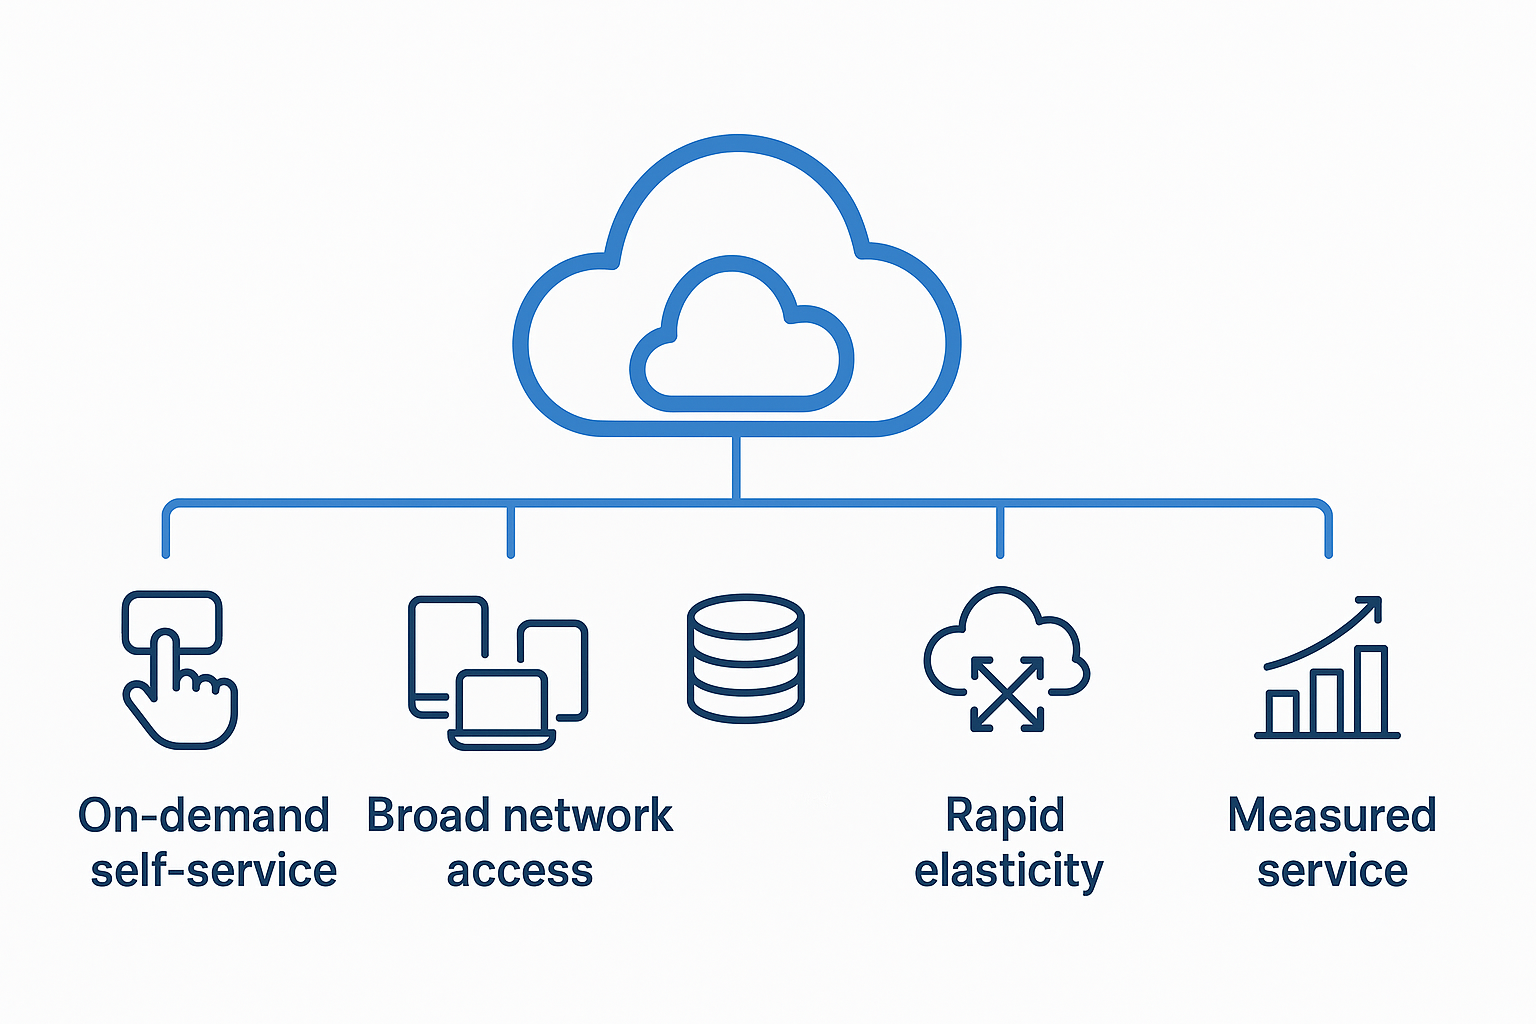
\includegraphics[width=0.7\textwidth]{Tong_quan_DTDM/Dac_diem_DTDM.png}
    \caption{Đặc điểm của điện toán đám mây}
    \label{fig:cloud_intro}
\end{figure}

\subsection{Ưu điểm và nhược điểm của hệ thống điện toán đám mây}
\begin{myitem}
\item Ưu điểm của dịch vụ lưu trữ đám mây:
  \begin{mysubitem}
  \item Tiết kiệm chi phí: Không cần đầu tư vào phần cứng lưu trữ vật lý, người dùng chỉ trả tiền cho dung lượng lưu trữ và dịch vụ mà họ thực sự sử dụng.
  \item Khả năng mở rộng linh hoạt: Dung lượng lưu trữ có thể dễ dàng tăng hoặc giảm theo nhu cầu mà không cần thay đổi cơ sở hạ tầng.
  \item Truy cập từ xa: Dữ liệu có thể được truy cập từ bất kỳ đâu qua internet, thuận tiện cho việc làm việc từ xa và chia sẻ tài liệu.
  \item Sao lưu và phục hồi dữ liệu: Nhiều dịch vụ lưu trữ đám mây cung cấp tính năng sao lưu tự động và phục hồi dữ liệu, giúp bảo vệ dữ liệu khỏi mất mát hoặc sự cố.
  \item Bảo mật và mã hóa: Các nhà cung cấp dịch vụ lưu trữ đám mây thường áp dụng các biện pháp bảo mật và mã hóa dữ liệu, giúp bảo vệ thông tin khỏi truy cập trái phép.
  \end{mysubitem}

\item Nhược điểm của dịch vụ lưu trữ đám mây:
  \begin{mysubitem}
  \item Vấn đề bảo mật và quyền riêng tư: Dữ liệu được lưu trữ trên máy chủ của bên thứ ba có thể gặp rủi ro về bảo mật và quyền riêng tư, đặc biệt nếu nhà cung cấp không có biện pháp bảo vệ đủ mạnh.
  \item Phụ thuộc vào kết nối internet: Truy cập và quản lý dữ liệu phụ thuộc vào kết nối internet, có thể gây khó khăn nếu kết nối không ổn định hoặc không có kết nối.
  \item Chi phí phát sinh: Mặc dù chi phí ban đầu thấp, nhưng việc lưu trữ dữ liệu lớn hoặc nhiều người dùng có thể dẫn đến chi phí phát sinh không lường trước được.
  \item Khó khăn trong quản lý dữ liệu lớn: Quản lý và tổ chức dữ liệu lớn có thể trở nên phức tạp, đặc biệt nếu không có các công cụ quản lý dữ liệu hiệu quả.
  \item Khả năng phụ thuộc vào nhà cung cấp: Doanh nghiệp có thể gặp khó khăn trong việc di chuyển dữ liệu hoặc ứng dụng nếu muốn chuyển sang nhà cung cấp khác hoặc đưa trở lại quản lý nội bộ.
  \end{mysubitem}
\end{myitem}

\subsection{Sơ lược các công nghệ ứng dụng trong điện toán đám mây}
\subsubsection{Công nghệ ảo hoá}
Công nghệ ảo hóa (virtualization) là công nghệ quan trọng nhất ứng dụng trong điện toán đám mây. Công nghệ ảo hóa là công nghệ cho phép tạo ra các thực thể ảo có tính năng tương đương như các thực thể vật lý, ví dụ như thiết bị lưu trữ, bộ vi xử lý,… Ảo hóa phần cứng (hardware virtualization) tham chiếu tới việc tạo ra các máy ảo (virtual machine) mà hoạt động với hệ điều hành được cài đặt như một máy tính vật lý thực. Ví dụ, một máy ảo chạy hệ điều hành Ubuntu có thể được tạo ra trên một máy tính thực cài hệ điều hành Windows.


Điều này được thể hiện qua việc có thể khởi tạo nhiều máy ảo với năng lực tính toán và năng lực lưu trữ bé hơn trên duy nhất một máy chủ vật lý. Máy chủ vật lý được gọi là host machine còn máy ảo (virtual machine) được gọi là máy khách (guest machine). Khái niệm "host" và "guest" được sử dụng để phân biệt phần mềm chạy trên máy tính vật lý hay phần mềm chạy trên máy ảo. Phần mềm hay firmware tạo máy ảo được gọi là hypervisor hay virtual machine manager.

Thông thường việc đầu tư cho một trung tâm công nghệ thông tin rất tốn kém. Chi phí mua các máy chủ cấu hình mạng và các phần mềm bản quyền rất là đắt. Vậy nên việc ảo hóa trở thành nhu cầu cần thiết cho bất kỳ doanh nghiệp nào. Bởi thay vì mua 10 máy chủ cho 10 ứng dụng thì chỉ cần mua một hai máy chủ có hỗ trợ ảo hóa vẫn có thể chạy tốt cả 10 ứng dụng. Điều này cho thấy sự khác biệt giữa hệ thống ảo hóa và không ảo hóa. Ngoài ra việc ảo hóa còn có các lợi ích sau:

\begin{myitem}
\item Quản lý đơn giản;

\item Tiển khai nhanh;

\item Phục hồi và lưu trữ hệ thống nhanh;

\item Cân bằng tải và phân phối tài nguyên linh hoạt;

\item Tiết kiệm chi phí;

\item Ảo hóa góp phần tăng cường tính liên tục, hạn chế ngắt quãng.
\end{myitem}

\subsubsection{Công nghệ tự động hóa giám sát điều phối tài nguyên (automation, dynamic dynamic orchestration)}
Công nghệ giám sát điều phối tài nguyên động là nền tảng để điện toán đám mây thực hiện cam kết chất lượng cung cấp dịch vụ điện toán. Với công nghệ điều phối tài nguyên động, việc lắp đặt thêm hay giảm bớt các tài nguyên máy chủ vật lý hoặc máy chủ lưu trữ dữ liệu được thực hiện tự động để hệ thống điện toán luôn đáp ứng được giao kèo trong hợp đồng dịch vụ đã ký với bên người sử dụng.

\subsubsection{Công nghệ tính toán phân tán, hệ phân tán}
Điện toán đám mây là một dạng hệ phân tán xuất phát từ yêu cầu cung ứng dịch vụ cho lượng người sử dụng khổng lồ. Tài nguyên tính toán của điện toán đám mây là tổng thể kết hợp của hạ tầng mạng và hàng nghìn máy chủ vật lý phân tán trên một hay nhiều trung tâm dữ liệu số (data centers).

\subsubsection{Công nghệ Web 2.0}
Web 2.0 là nền tảng công nghệ phát triển các sản phẩm ứng dụng hướng dịch vụ trên nền điện toán đám mây. Công nghệ Web 2.0 phát triển cho phép phát triển giao diện ứng dụng web dễ dàng và nhanh chóng và trên nhiều thiết bị giao diện khác nhau. Web 2.0 phát triển làm xóa đi khoảng cách về thiết kế giao diện giữa ứng dụng máy tính thông thường và ứng dụng trên nền web, cho phép chuyển hóa ứng dụng qua dịch vụ trên nền điện toán đám mây mà không ảnh hưởng đến thói quen người sử dụng.

\subsection{Một số đám mây được triển khai phổ biến hiện nay}
Hiện nay, các đám mây được chia thành hai nhóm:

\begin{myitem}
\item Thứ nhất, Ba “Hyperscaler” hàng đầu (Thị phần toàn cầu lớn nhất):
  \begin{mysubitem}
  \item Amazon Web Services (AWS): Dẫn đầu thị trường với khoảng 29--32\% thị phần toàn cầu quý 1 năm 2025, AWS sở hữu hệ sinh thái dịch vụ phong phú (hơn 200 dịch vụ), vùng hoạt động rộng khắp toàn cầu và năng lực hỗ trợ AI nổi bật.
  
  \item Microsoft Azure: Xếp thứ hai, chiếm khoảng 22 - 24\% thị phần, Azure mạnh ở mảng tích hợp với hệ sinh thái Microsoft (365, Active Directory\ldots), hỗ trợ hybrid cloud tốt (Azure Arc, Stack) và được doanh nghiệp lớn ưa chuộng.
  
  \item Google Cloud Platform (GCP): Đứng thứ ba với khoảng 12\% thị phần toàn cầu, GCP nổi bật về năng lực trong AI/ML, phân tích dữ liệu (BigQuery, Vertex AI), container hoá (Kubernetes), và được đánh giá cao bởi các startup \& tech-savvy teams.
  \end{mysubitem}

\begin{figure}[H] % cần gói float nếu muốn fix vị trí
    \centering
    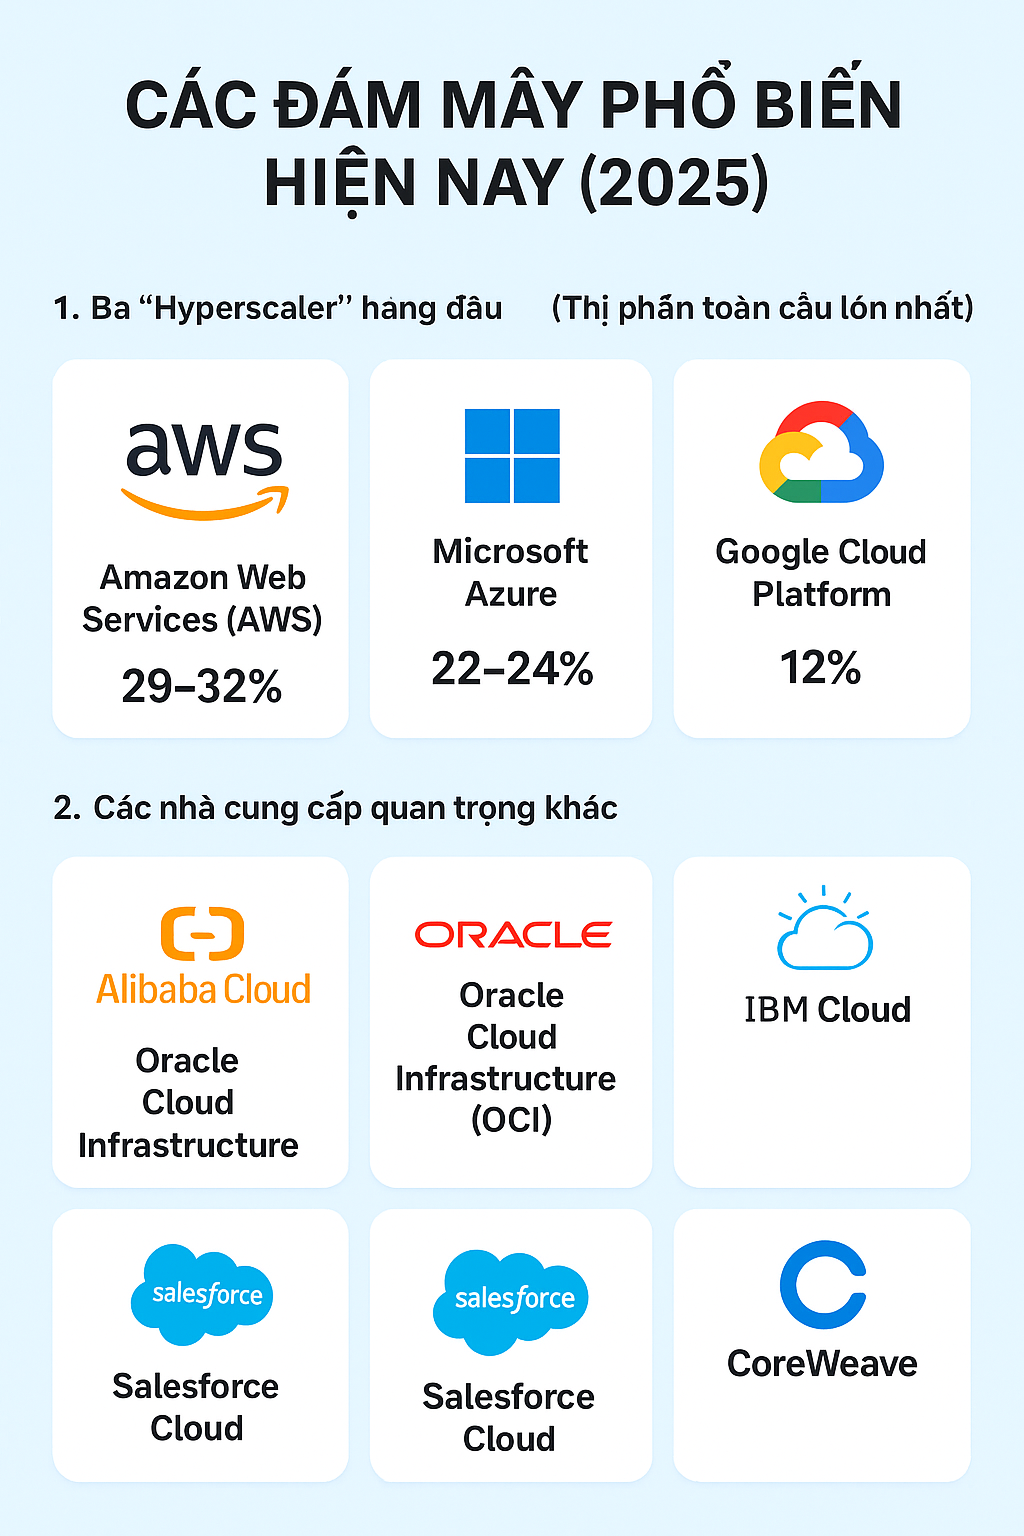
\includegraphics[width=0.7\textwidth]{Tong_quan_DTDM/Cac_dam_may_pho_bien.png}
    \caption{Các đám mây được triển khai phổ biến hiện nay}
    \label{fig:cloud_intro}
\end{figure}


\item Thứ hai, Các nhà cung cấp quan trọng khác:
  \begin{mysubitem}
  \item Alibaba Cloud - Khoảng 4\% thị phần toàn cầu, đặc biệt mạnh ở khu vực Châu Á -- Thái Bình Dương.
  
  \item Oracle Cloud Infrastructure (OCI) -- Chiếm 3\% thị phần, phát triển nhanh với nền tảng tối ưu hiệu năng cao, đặc biệt cho các hệ thống Oracle truyền thống.
  
  \item Tencent Cloud -- Khoảng 2\% thị phần toàn cầu, nhưng là nhà cung cấp lớn thứ ba tại Trung Quốc với khoảng 15\% nội địa. Phát triển mạnh ở Đông Nam Á.
  
  \item Các nhà cung cấp khác như OVHcloud, DigitalOcean, Linode, Kamatera\ldots\ nổi bật ở mảng nhỏ và vừa, developer-friendly, hoặc phục vụ nhu cầu địa phương/chi phí thấp.
  \end{mysubitem}
\end{myitem}

\subsection{Các loại hình dịch vụ}
Điện toán đám mây có ba mô hình cung cấp dịch vụ, tùy theo các đối tượng khách hàng như sau \cite{vngcloud_iaas_paas_saas}:

\begin{myitem}
\item Infrastructure as a Service – Dịch vụ hạ tầng

\item Platform as a Service – Dịch vụ nền tảng

\item Software as a Service – Dịch vụ phần mềm

\end{myitem}

\begin{figure}[H] % cần gói float nếu muốn fix vị trí
    \centering
    
\includegraphics[width=0.7\textwidth]{Tong_quan_DTDM/Cac_loai_hinh_dich_vu.jpg}
    \caption{Mỗi mô hình cung cấp các mức độ quản lý và chức năng khác nhau, cho
phép doanh nghiệp lựa chọn mô hình phù hợp nhất với nhu cầu}
    \label{fig:cloud_intro}
\end{figure}

\subsubsection{Infrastructure as a Service (IaaS)}
\begin{myitem}
  \item \textbf{Định nghĩa:} Cung cấp cơ sở hạ tầng công nghệ thông tin như máy chủ, lưu trữ và mạng qua đám mây.

  \item \textbf{Quyền kiểm soát:} Người dùng có toàn quyền quản lý cơ sở hạ tầng, hệ điều hành, ứng dụng.

  \item \textbf{Đối tượng sử dụng:} Doanh nghiệp cần kiểm soát và tùy chỉnh hạ tầng theo nhu cầu riêng.

  \item \textbf{Ưu điểm:}
    \begin{mysubitem}
      \item Doanh nghiệp có thể thiết kế, điều chỉnh cơ sở hạ tầng theo nhu cầu.
      \item Tiết kiệm chi phí mua phần cứng.
      \item Dễ dàng mở rộng hoặc thu hẹp tài nguyên theo sự phát triển của doanh nghiệp.
      \item Người dùng có quyền quản lý toàn bộ hệ điều hành và ứng dụng.
    \end{mysubitem}

  \item \textbf{Nhược điểm:} Yêu cầu có chuyên môn kỹ thuật, có đội ngũ công nghệ thông tin để quản lý và bảo trì.
\end{myitem}

\begin{figure}[H] % cần gói float nếu muốn fix vị trí
    \centering
    
\includegraphics[width=0.7\textwidth]{Tong_quan_DTDM/IaaS.jpg}
    \caption{Nhà cung cấp IaaS có trách nhiệm trong việc bảo mật cơ sở hạ tầng
dành riêng cho ứng dụng điện toán đám mây}
    \label{fig:cloud_intro}
\end{figure}

\subsubsection{Platform as a Service (PaaS)}
\begin{myitem}
  \item \textbf{Định nghĩa:} Cung cấp nền tảng phát triển và triển khai ứng dụng mà không cần quản lý hạ tầng.

  \item \textbf{Quyền kiểm soát:} Người dùng quản lý ứng dụng nhưng không kiểm soát cơ sở hạ tầng.

  \item \textbf{Đối tượng sử dụng:} Các nhà phát triển muốn tập trung vào viết mã mà không lo về cơ sở hạ tầng.

  \item \textbf{Ưu điểm:}
    \begin{mysubitem}
      \item Không cần bảo trì và cập nhật hệ thống máy chủ.
      \item Nhà phát triển có thể tập trung vào viết mã và ứng dụng.
      \item PaaS cung cấp các công cụ sẵn có giúp giảm thời gian phát triển ứng dụng.
      \item Tạo điều kiện cho việc hợp tác giữa các thành viên nhóm phát triển.
    \end{mysubitem}

  \item \textbf{Nhược điểm:} Khả năng kiểm soát cơ sở hạ tầng bị hạn chế, phải phụ thuộc vào nhà cung cấp.
\end{myitem}

\begin{figure}[H] % cần gói float nếu muốn fix vị trí
    \centering
    
\includegraphics[width=0.9\textwidth]{Tong_quan_DTDM/PaaS.jpg}
    \caption{PaaS là mô hình dịch vụ điện toán đám mây trong đó nhà cung cấp bên
thứ ba cung cấp các công cụ phần cứng và phần mềm cho người dùng thông qua
Internet}
    \label{fig:cloud_intro}
\end{figure}

\subsubsection{Software as a Service (SaaS)}
\begin{myitem}
  \item \textbf{Định nghĩa:} Cung cấp phần mềm hoàn chỉnh thông qua internet mà không cần cài đặt.

  \item \textbf{Quyền kiểm soát:} Người dùng chỉ sử dụng phần mềm, nhà cung cấp quản lý toàn bộ.

  \item \textbf{Đối tượng sử dụng:} Người dùng cuối (End User) hoặc doanh nghiệp cần phần mềm để sử dụng ngay.

  \item \textbf{Ưu điểm:}
    \begin{mysubitem}
      \item Phần mềm có sẵn để sử dụng ngay qua internet mà không cần cài đặt.
      \item Nhà cung cấp dịch vụ chịu trách nhiệm quản lý, cập nhật và bảo mật phần mềm.
      \item Không cần chi phí phát triển hoặc quản lý phần mềm.
      \item Người dùng có thể sử dụng phần mềm với bất kỳ thiết bị nào có kết nối internet.
    \end{mysubitem}

  \item \textbf{Nhược điểm:} Khả năng tùy chỉnh hạn chế, phụ thuộc vào nhà cung cấp dịch vụ.
\end{myitem}

\begin{figure}[H] % cần gói float nếu muốn fix vị trí
    \centering
    
\includegraphics[width=0.7\textwidth]{Tong_quan_DTDM/SaaS.jpg}
    \caption{SaaS cung cấp sự lựa chọn về phần mềm và bảo trì của bên thứ
ba toàn diện nhất}
    \label{fig:cloud_intro}
\end{figure}

\subsection{Xử lý dữ liệu phân tán}
\begin{myitem}
  \item NFS (Network File System): Cho phép chia sẻ tập tin cho nhiều người dùng trên cùng mạng và người dùng có thể thao tác như với tập tin trên chính đĩa cứng của mình.

  \item AFS (Andrew File System): Hệ thống tập tin phân tán nhằm mục đích chia sẻ tập tin cho một lượng lớn người dùng mạng. So với NFS, AFS có tính khả mở cao hơn, đáp ứng được số lượng người dùng lớn hơn nhờ cơ chế sau:
    \begin{mysubitem}
      \item Khi truy cập tập tin, toàn bộ tập tin sẽ được sao chép về phía máy người sử dụng và các thao tác đọc/ghi được thực hiện trên tập tin đó.
      \item Khi tập tin được đóng, nội dung tập tin sẽ được cập nhật về phía máy chủ lưu trữ. Do đó, quá trình đọc/ghi đồng thời là trong suốt đối với từng người dùng, nhưng tính nhất quán của tập tin không được đảm bảo.
    \end{mysubitem}

  \item GFS (Google File System): Hệ thống tệp phân tán của Google, được thiết kế để lưu trữ và xử lý dữ liệu lớn, tối ưu cho các tác vụ đọc/ghi dữ liệu lớn và hỗ trợ độ bền cao.

\begin{figure}[H] % cần gói float nếu muốn fix vị trí
    \centering
    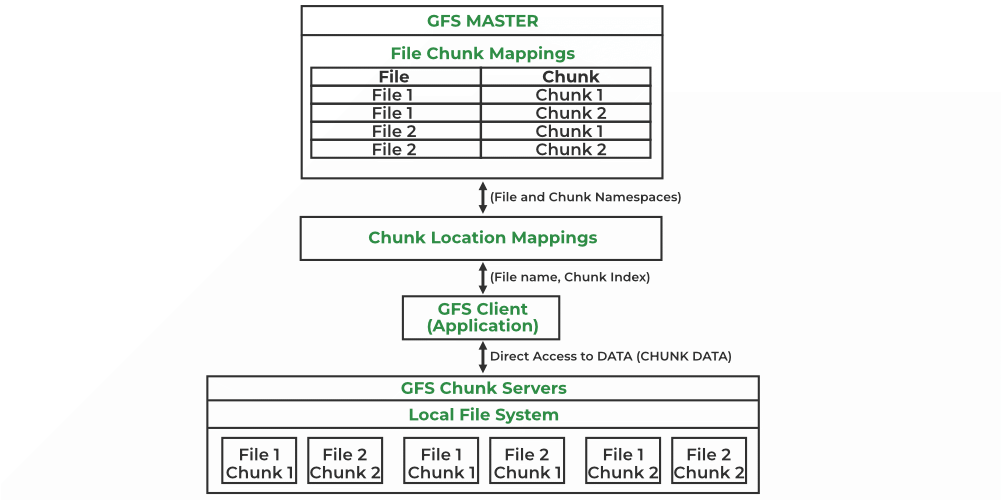
\includegraphics[width=0.9\textwidth]{Tong_quan_DTDM/GFS.png}
    \caption{Google File System}
    \label{fig:cloud_intro}
\end{figure}

  \item HDFS (Hadoop Distributed File System): Hệ thống tệp phân tán dùng trong Apache Hadoop, cho phép lưu trữ và xử lý dữ liệu lớn trên nhiều máy tính. HDFS được tối ưu cho xử lý dữ liệu phân tán, chịu lỗi tốt và có khả năng mở rộng.

  \item RDBMS (Relational Database Management System): Hệ quản trị cơ sở dữ liệu quan hệ, sử dụng bảng để lưu trữ dữ liệu và hỗ trợ các truy vấn SQL để xử lý dữ liệu.  
  Ví dụ: MySQL, PostgreSQL.

  \item NoSQL: Cơ sở dữ liệu phi quan hệ, không sử dụng bảng và SQL, thích hợp cho ứng dụng yêu cầu xử lý dữ liệu phi cấu trúc và có khả năng mở rộng cao.  
  Ví dụ: MongoDB, Cassandra.
\end{myitem}

\subsection{Mô hình triển khai hệ thống điện toán đám mây}
\begin{myitem}
  \item Public Cloud (Đám mây “công cộng”)  

  \hspace*{1cm}Public Cloud là mô hình đám mây do bên thứ ba (các nhà cung cấp dịch vụ đám mây như AWS, Microsoft Azure, Google Cloud, IBM Cloud, v.v.) cung cấp và quản lý. Các dịch vụ này được triển khai trên hạ tầng nằm ngoài tường lửa của doanh nghiệp và được chia sẻ cho nhiều người dùng hoặc tổ chức khác nhau. Người dùng sẽ đăng ký và trả phí sử dụng theo chính sách giá của nhà cung cấp, thường dựa trên mức tiêu thụ tài nguyên (pay-as-you-go) \cite{aws_public_vs_private_cloud}..  

  \hspace*{1cm}Ưu điểm của mô hình này là tính linh hoạt, khả năng mở rộng gần như vô hạn, tiết kiệm chi phí đầu tư ban đầu và dễ dàng tiếp cận. Đây là mô hình phổ biến nhất hiện nay, phù hợp với các cá nhân, doanh nghiệp vừa và nhỏ, hoặc các tổ chức cần triển khai dịch vụ nhanh chóng mà không muốn đầu tư nhiều vào cơ sở hạ tầng.  

  \item Private Cloud (Đám mây “doanh nghiệp”) 

  \hspace*{1cm}Private Cloud được xây dựng và triển khai riêng biệt cho một doanh nghiệp hoặc tổ chức, thường nằm trong hệ thống mạng nội bộ và được bảo vệ bởi tường lửa. Việc quản lý và vận hành có thể do chính doanh nghiệp thực hiện hoặc thuê đối tác chuyên trách \cite{aws_public_vs_private_cloud}.  

  \hspace*{1cm}Điểm mạnh của mô hình này là tính bảo mật cao, khả năng kiểm soát toàn diện và khả năng tùy chỉnh hạ tầng theo nhu cầu riêng. Private Cloud phù hợp với các tổ chức lớn, cơ quan chính phủ, ngân hàng, tài chính, hoặc những đơn vị có yêu cầu nghiêm ngặt về bảo mật dữ liệu. Tuy nhiên, chi phí đầu tư và bảo trì hệ thống thường cao hơn so với Public Cloud.  

  \item Hybrid Cloud (Đám mây “lai”)  

  \hspace*{1cm}Hybrid Cloud là sự kết hợp giữa Public Cloud và Private Cloud, tạo nên một mô hình linh hoạt, giúp doanh nghiệp tận dụng được lợi thế của cả hai. Doanh nghiệp có thể triển khai các dịch vụ quan trọng, yêu cầu bảo mật cao trên Private Cloud, trong khi tận dụng Public Cloud để mở rộng năng lực xử lý hoặc lưu trữ khi có nhu cầu đột biến.  

  \hspace*{1cm}Mô hình này mang lại sự cân bằng giữa hiệu quả chi phí, khả năng mở rộng và mức độ an toàn dữ liệu. Việc quản lý Hybrid Cloud thường đòi hỏi sự phối hợp giữa doanh nghiệp và nhà cung cấp dịch vụ đám mây công cộng, cùng với các giải pháp đồng bộ dữ liệu và bảo mật phức tạp hơn.  

   \item Community Cloud (Đám mây cộng đồng) 

  \hspace*{1cm}Community Cloud được xây dựng và chia sẻ bởi nhiều tổ chức hoặc doanh nghiệp có cùng mục tiêu, nhu cầu, hoặc mối quan tâm chung, ví dụ như các trường đại học, viện nghiên cứu, bệnh viện, tổ chức tài chính. Hạ tầng đám mây cộng đồng có thể do chính các đơn vị tham gia cùng quản lý hoặc ủy thác cho bên thứ ba.
  
  \hspace*{1cm}Mô hình này mang lại sự cân bằng giữa tính riêng tư của Private Cloud và tính chia sẻ của Public Cloud, đồng thời tối ưu chi phí khi nhiều tổ chức cùng đầu tư và sử dụng chung. Tuy nhiên, việc quản lý và phân chia quyền hạn, trách nhiệm giữa các bên tham gia đòi hỏi cơ chế rõ ràng để tránh xung đột lợi ích.
\end{myitem}

\newpage
\subsection*{\centering KẾT LUẬN CHƯƠNG 1}
\addcontentsline{toc}{subsection}{KẾT LUẬN CHƯƠNG 1}
Chương 1 đã cung cấp một cái nhìn tổng quan về điện toán đám mây, từ khái niệm, lịch sử hình thành, đến các đặc điểm, ưu nhược điểm, công nghệ nền tảng, mô hình triển khai và các loại dịch vụ phổ biến. Điện toán đám mây được hình thành từ ý tưởng chia sẻ tài nguyên tính toán trên các máy chủ lớn và phát triển mạnh mẽ nhờ khả năng cung cấp tài nguyên linh hoạt, truy cập từ xa, tiết kiệm chi phí và mở rộng quy mô dễ dàng.

Các đặc tính cốt lõi của điện toán đám mây gồm: tự phục vụ theo yêu cầu, truy cập mạng rộng rãi, tập trung tài nguyên, tính mềm dẻo và dịch vụ đo lường. Đồng thời, chương cũng phân tích ưu nhược điểm của hệ thống đám mây, từ khả năng tiết kiệm chi phí, mở rộng linh hoạt, truy cập từ xa đến những hạn chế về bảo mật, phụ thuộc kết nối mạng và chi phí phát sinh.

Chương này cũng trình bày các công nghệ nền tảng hỗ trợ điện toán đám mây như ảo hóa, tự động hóa giám sát và điều phối tài nguyên, tính toán phân tán và Web 2.0, cùng với các hệ thống lưu trữ và cơ sở dữ liệu phân tán giúp xử lý dữ liệu hiệu quả. Bên cạnh đó, các mô hình triển khai đám mây phổ biến gồm Public Cloud, Private Cloud, Hybrid Cloud và Community Cloud, cùng ba loại hình dịch vụ chính IaaS, PaaS và SaaS, đều được giới thiệu để người dùng có thể lựa chọn giải pháp phù hợp với nhu cầu.

Tóm lại, chương 1 tạo nền tảng kiến thức cơ bản và toàn diện về điện toán đám mây, giúp nhận thức được tiềm năng ứng dụng, các lợi ích và thách thức, đồng thời cung cấp cơ sở lý thuyết quan trọng để triển khai các nghiên cứu và ứng dụng thực tiễn trong các chương tiếp theo.
\newpage

\section{CÔNG NGHỆ ẢO HÓA CỦA ORACLE CLOUD}
\subsection{Khái niệm về ảo hóa}
Ảo hóa (Virtualization) là một công nghệ tiên tiến cho phép tạo ra các phiên bản ảo của tài nguyên phần cứng hoặc phần mềm, chẳng hạn như máy chủ, bộ nhớ, thiết bị lưu trữ, hệ điều hành hay mạng máy tính. Thay vì phải triển khai nhiều thiết bị vật lý tách biệt, ảo hóa sử dụng phần mềm trung gian (thường gọi là hypervisor) để mô phỏng và quản lý các chức năng phần cứng, từ đó cho phép nhiều máy ảo (Virtual Machine – VM) hoạt động song song trên cùng một máy chủ vật lý.

Trong môi trường ảo hóa, mỗi máy ảo hoạt động độc lập như một hệ thống riêng biệt, có hệ điều hành, ứng dụng và tài nguyên được phân bổ riêng. Điều này mang lại sự linh hoạt và hiệu quả cao trong việc sử dụng tài nguyên. Thay vì để một máy chủ vật lý chỉ chạy một ứng dụng và gây lãng phí tài nguyên, công nghệ ảo hóa giúp hợp nhất nhiều ứng dụng, dịch vụ trên cùng một hạ tầng phần cứng mà vẫn đảm bảo tính bảo mật, ổn định và hiệu năng.

Đối với doanh nghiệp, ảo hóa mang lại nhiều lợi ích to lớn: tối ưu hóa chi phí đầu tư phần cứng, giảm chi phí vận hành và bảo trì, tăng khả năng mở rộng, đồng thời nâng cao hiệu quả quản lý hệ thống công nghệ thông tin. Ngoài ra, công nghệ này cũng đóng vai trò nền tảng cho điện toán đám mây (Cloud Computing), cho phép triển khai các dịch vụ lưu trữ, điện toán, phân tích dữ liệu và ứng dụng doanh nghiệp trên quy mô lớn một cách linh hoạt.

Nhờ ảo hóa, các tổ chức có thể dễ dàng sao lưu, khôi phục dữ liệu, tạo môi trường kiểm thử – phát triển phần mềm an toàn mà không ảnh hưởng đến hệ thống chính, cũng như triển khai hạ tầng công nghệ thông tin theo mô hình dịch vụ (IT as a Service – ITaaS). Có thể nói, ảo hóa không chỉ giúp tận dụng tối đa sức mạnh của phần cứng mà còn góp phần thay đổi cách các doanh nghiệp xây dựng và vận hành hạ tầng số trong thời đại công nghệ 4.0.

\subsection{Một số kiến trúc ảo hóa}
\subsubsection{Hosted-based Virtualization (Ảo hóa dựa trên hệ điều hành nền tảng)}
 Đây là kiến trúc ảo hóa trong đó hypervisor (phần mềm ảo hóa) được cài đặt trên hệ điều hành chính (host OS). Điều đó có nghĩa là máy chủ phải cài đặt hệ điều hành trước, sau đó mới cài đặt hypervisor để tạo và quản lý các máy ảo (VM).

\begin{figure}[H] % cần gói float nếu muốn fix vị trí
    \centering
    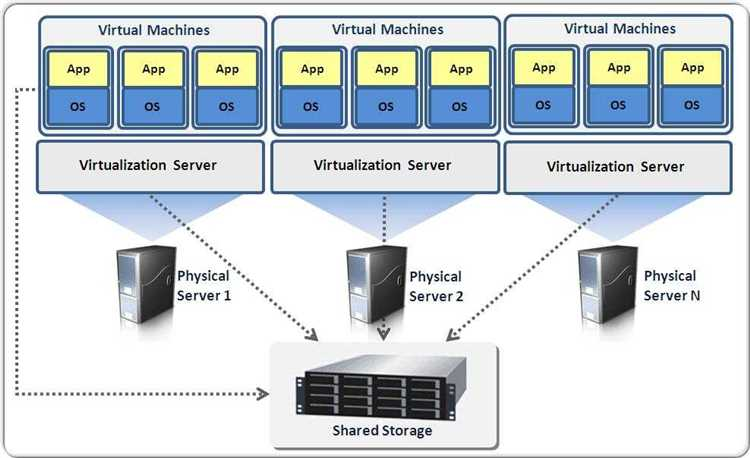
\includegraphics[width=0.9\textwidth]{Oracle_cloud/Hosted-based-Virtualization.jpg}
    \caption{Hosted-based Virtualization}
    \label{fig:cloud_intro}
\end{figure}

\begin{myitem}
\item Ưu điểm:
  \begin{mysubitem}
  \item Cài đặt và triển khai dễ dàng, thân thiện với người dùng.
  
  \item Phù hợp cho môi trường thử nghiệm, phát triển ứng dụng hoặc máy tính cá nhân.
  
  \item Có thể chạy nhiều hệ điều hành khác nhau trên cùng một máy.
  
  \end{mysubitem}

\item Nhược điểm:

  \begin{mysubitem}
  \item Hiệu năng thấp hơn vì hypervisor phải phụ thuộc và hoạt động gián tiếp thông qua hệ điều hành nền tảng.
  
  \item Ít phù hợp cho môi trường doanh nghiệp lớn hoặc hệ thống yêu cầu hiệu suất cao.

  \end{mysubitem}

\item Ví dụ: VMware Workstation, Oracle VirtualBox, Microsoft Virtual PC.
\end{myitem}

\subsection{Công nghệ ảo hóa máy chủ của Oracle cloud}
Oracle VM Server là một giải pháp ảo hóa máy chủ được Oracle phát triển, dựa trên nền tảng Xen Hypervisor nhưng đã được cải tiến và tích hợp chặt chẽ với Linux kernel nhằm tối ưu hóa hiệu suất và khả năng quản lý. Đây là một trong những sản phẩm chủ lực trong hệ sinh thái Oracle Virtualization, hỗ trợ triển khai các ứng dụng và dịch vụ doanh nghiệp trên hạ tầng ảo hóa mạnh mẽ, ổn định.

\begin{figure}[H] % cần gói float nếu muốn fix vị trí
    \centering
    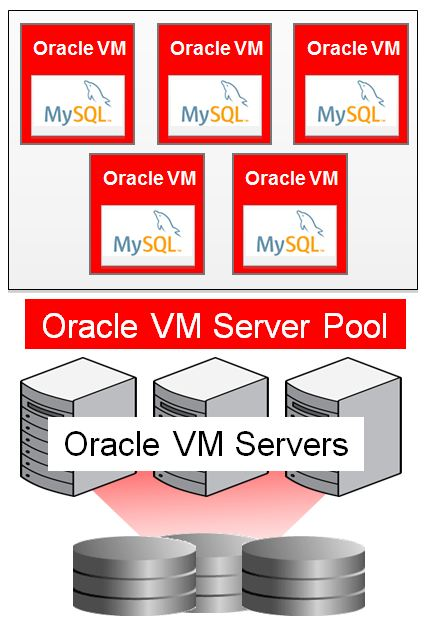
\includegraphics[width=0.65\textwidth]{Oracle_cloud/Oracle_VM_Server.jpg}
    \caption{Oracle VM Server}
    \label{fig:cloud_intro}
\end{figure}

Đặc điểm nổi bật:

\begin{myitem}
\item Dựa trên Xen Hypervisor nâng cao: Oracle VM Server sử dụng Xen – một công nghệ ảo hóa mã nguồn mở phổ biến, nhưng được Oracle tùy biến để đạt hiệu năng và độ ổn định cao hơn.


\item Hỗ trợ phần cứng và phần mềm phong phú: Có thể hoạt động với nhiều loại thiết bị, hệ thống file khác nhau, đồng thời tích hợp với phần mềm quản lý RAID để tăng cường khả năng bảo vệ dữ liệu.


\item Trình ảo hóa nhẹ và bảo mật: Hypervisor trong Oracle VM Server là thực thể duy nhất có đặc quyền cao nhất trong hệ thống, chiếm dung lượng rất nhỏ, giúp giảm thiểu nguy cơ tấn công và tối ưu tài nguyên.


\item Quản lý tài nguyên cơ bản: Oracle VM Server trực tiếp quản lý các thành phần quan trọng của hệ thống như CPU, bộ nhớ, quyền đặc biệt (privileges), và xử lý ngắt phần cứng (hardware interrupts).


\item Khả năng trừu tượng hóa cao: Thay vì chỉ gắn liền với phần cứng cụ thể, Oracle VM Server cung cấp lớp trừu tượng cho phép thực hiện cùng một tác vụ logic trên nhiều loại máy chủ vật lý khác nhau. Điều này mang lại sự linh hoạt trong triển khai và di chuyển khối lượng công việc.
\end{myitem}

Lợi ích khi sử dụng
\begin{myitem}
\item Hiệu năng cao: Nhờ quản lý trực tiếp tài nguyên phần cứng mà không cần thông qua hệ điều hành trung gian.

\item Khả năng mở rộng: Hỗ trợ triển khai trên nhiều máy chủ vật lý, dễ dàng mở rộng hệ thống khi nhu cầu tăng.


\item Tích hợp sâu với hệ sinh thái Oracle: Đặc biệt tối ưu cho cơ sở dữ liệu Oracle, Middleware, và các ứng dụng doanh nghiệp khác.


\item Bảo mật và ổn định: Cơ chế phân tách tài nguyên rõ ràng giúp giảm nguy cơ ảnh hưởng lẫn nhau giữa các máy ảo.

\end{myitem}

\subsubsection{Chức năng của máy chủ VM Oracle}
\subsubsubsection{Server Pool Master}
\begin{myitem}
\item Đây là máy chủ trung tâm trong một Server Pool (nhóm máy chủ).
\item Tất cả các hoạt động quản lý trong pool đều xoay quanh Server Pool Master, nó giữ vai trò:
  \begin{mysubitem}
  \item Điểm liên lạc giữa nhóm máy chủ với Oracle VM Manager.
  
  \item Điều phối hoạt động của các Oracle VM Server khác trong nhóm, đảm bảo tài nguyên được phân bổ hợp lý.
  
  \item Quản lý siêu dữ liệu (metadata) của Server Pool, bao gồm thông tin về cấu hình máy ảo, phân quyền, chính sách tài nguyên.

  \end{mysubitem}

\item Nếu Server Pool Master gặp sự cố, Oracle VM có thể bầu chọn hoặc chỉ định một máy chủ khác thay thế để duy trì hoạt động.
\end{myitem}

\subsubsubsection{Utility Server}
\begin{myitem}
\item Đây là loại máy chủ có chức năng chuyên dụng trong việc tạo, triển khai và xóa các máy ảo.

\item Nhiệm vụ chính bao gồm:

  \begin{mysubitem}
  \item Tạo mới hoặc clone máy ảo dựa trên các template.
  
  \item Xóa máy ảo khi không còn sử dụng.
  
  \item Quản lý Oracle VM Templates, Virtual Appliances và Server Pools.

  \end{mysubitem}

\item Utility Server thường được dùng trong giai đoạn triển khai, cài đặt, hoặc khi có nhu cầu mở rộng hệ thống nhanh chóng.

\end{myitem}

\subsubsubsection{Virtual Machine Server}
\begin{myitem}
\item Đây là máy chủ chịu trách nhiệm trực tiếp chạy các máy ảo (Virtual Machines – VM).

\item Vai trò chính:

  \begin{mysubitem}
  \item Cung cấp môi trường thực thi cho các ứng dụng và dịch vụ chạy trong máy ảo.
  
  \item Quản lý việc phân bổ tài nguyên phần cứng (CPU, RAM, lưu trữ, mạng) cho các VM.

  \item Đảm bảo tính ổn định và hiệu năng của hệ thống trong quá trình vận hành.

  \end{mysubitem}

\item Đây là thành phần chủ lực trong hạ tầng Oracle VM vì nó gánh vác công việc thực tế của doanh nghiệp.
\item Oracle VM VirtualBox là một hosted hypervisor tự do nguồn mở phát triền bởi Oracle \cite{spca_vm_virtualbox}.

\end{myitem}

\begin{figure}[H] % cần gói float nếu muốn fix vị trí
    \centering
    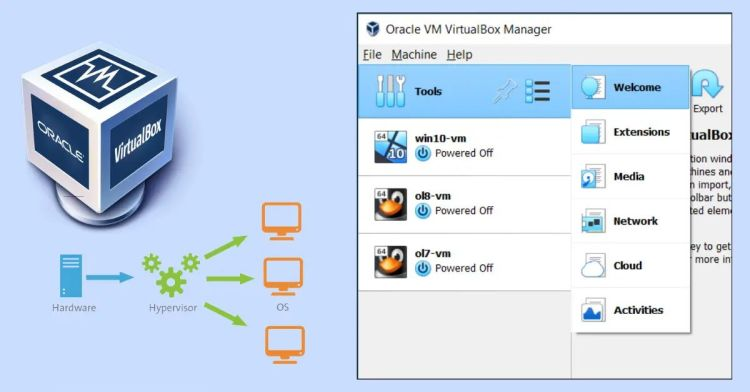
\includegraphics[width=1.0\textwidth]{Oracle_cloud/virtualbox.jpg}
    \caption{Oracle VM VirtualBox}
    \label{fig:cloud_intro}
\end{figure}

\subsubsection{Đặc điểm của Oracle VM Server}
Oracle VM Server không chỉ đáp ứng đầy đủ các chức năng cơ bản của một nền tảng ảo hóa, mà còn sở hữu những tính năng nâng cao, giúp nó trở thành một trong những giải pháp mạnh mẽ và khác biệt trên thị trường.

\begin{myitem}

\item Tính sẵn sàng cao (High Availability – HA)

\hspace*{1cm} Oracle VM Server được thiết kế với cơ chế tự động khởi động lại các máy ảo bị lỗi trên các máy chủ khác trong cùng Server Pool. Khi một máy chủ gặp sự cố, các máy ảo đang chạy trên đó sẽ được chuyển sang máy chủ khác một cách tự động, giúp giảm thiểu thời gian chết và đảm bảo dịch vụ vẫn hoạt động liên tục.

\hspace*{1cm} Điều này đặc biệt quan trọng trong môi trường trung tâm dữ liệu hoặc các ứng dụng doanh nghiệp yêu cầu tính liên tục cao, nơi bất kỳ gián đoạn nào cũng có thể ảnh hưởng đến hoạt động kinh doanh hoặc gây mất dữ liệu quan trọng. Nhờ tính năng HA, Oracle VM Server giúp doanh nghiệp yên tâm vận hành các ứng dụng quan trọng mà không lo gián đoạn.

\item Khả năng mở rộng và hiệu suất mạnh mẽ

\hspace*{1cm} Oracle VM Server dựa trên kiến trúc Xen Hypervisor tối ưu, giúp đạt hiệu suất cao nhưng vẫn giữ chi phí hợp lý. Nó có khả năng hỗ trợ lên tới 384 CPU vật lý và 6TB RAM, đáp ứng nhu cầu xử lý khối lượng công việc lớn trong môi trường đám mây và doanh nghiệp.

\hspace*{1cm} Đối với mỗi máy ảo, người dùng có thể cấu hình tới 256 CPU ảo và 2TB RAM. Với cấu hình này, Oracle VM Server có thể chạy mượt các ứng dụng phức tạp như ERP, CRM hoặc các hệ thống phân tích dữ liệu lớn (Big Data). Điều này giúp doanh nghiệp triển khai các dịch vụ nặng mà không lo thiếu tài nguyên, đồng thời tối ưu hóa hiệu quả vận hành.

\item Quản lý tập trung và nâng cao mà không tốn thêm chi phí

\hspace*{1cm} Oracle VM Server đi kèm với Oracle VM Manager, cung cấp giao diện quản lý tập trung dựa trên trình duyệt web. Người quản trị có thể dễ dàng quản lý các tài nguyên như máy ảo, nhóm máy chủ, lưu trữ và mạng, đồng thời theo dõi sự kiện và tình trạng hệ thống theo thời gian thực.

\hspace*{1cm} Nhờ tính năng quản lý tập trung này, doanh nghiệp không cần đầu tư thêm các công cụ quản lý bên ngoài. Việc phân bổ và giám sát tài nguyên trở nên hiệu quả hơn, giúp tiết kiệm chi phí vận hành và tránh phụ thuộc vào phần mềm thứ ba. Điều này đặc biệt hữu ích với các doanh nghiệp muốn duy trì hiệu quả vận hành mà vẫn kiểm soát chi phí.

\item Hỗ trợ đa dạng hệ điều hành

\hspace*{1cm} Oracle VM Server có thể chạy nhiều hệ điều hành khác nhau, bao gồm Oracle Linux, Oracle Solaris, Enterprise Linux, SUSE Linux Enterprise, Red Hat Enterprise Linux (RHEL), CentOS và các phiên bản phổ biến của Microsoft Windows.

\hspace*{1cm} Khả năng này giúp doanh nghiệp triển khai hạ tầng đa nền tảng mà vẫn đồng bộ trong cùng một hệ thống ảo hóa. Nhờ đó, các ứng dụng trên nhiều hệ điều hành khác nhau có thể cùng vận hành hiệu quả, nâng cao tính linh hoạt và khả năng tương thích của hạ tầng công nghệ thông tin.

\item Chuyển đổi máy ảo an toàn (Secure Live VM Migration)

\hspace*{1cm}Oracle VM Server hỗ trợ di chuyển trực tiếp các máy ảo đang chạy (live migration) từ máy chủ này sang máy chủ khác mà không gây gián đoạn dịch vụ. Quá trình di chuyển được thực hiện thông qua SSL URL an toàn, bảo vệ dữ liệu và kết nối trong suốt quá trình.

\hspace*{1cm} Tính năng này rất hữu ích khi doanh nghiệp cần bảo trì hệ thống theo kế hoạch hoặc mở rộng, tái phân bổ tài nguyên. Nhờ đó, dịch vụ luôn hoạt động liên tục, người dùng cuối không bị gián đoạn, giúp tăng tính ổn định và độ tin cậy của toàn bộ hệ thống.
\end{myitem}

\subsubsection{Ưu điểm – hạn chế của Oracle VM Server}
\begin{myitem}
\item Ưu điểm.

  \begin{mysubitem}
    \item Oracle VM hỗ trợ đa dạng nền tảng, tương thích với cả máy chủ x86 lẫn hệ điều hành Solaris. Ngoài ra, công cụ này còn cho phép nhân bản máy ảo (VM cloning), giúp triển khai nhanh chóng các hệ thống mới mà không cần cấu hình từ đầu, tiết kiệm đáng kể thời gian và công sức cho các quản trị viên.
    
    \item Về khả năng quản lý, Oracle VM cung cấp Oracle VM Manager với cả giao diện dòng lệnh (CLI) và Web Services API (WS-API). Điều này cho phép mức độ tự động hóa cao, giúp dễ dàng tích hợp Oracle VM với các hệ thống quản lý công nghệ thông tin khác, từ đó tối ưu hóa việc giám sát và vận hành hạ tầng ảo.
    
    \item Quá trình cài đặt và cấu hình Oracle VM cũng khá đơn giản, không đòi hỏi nhiều bước phức tạp. Điều này giúp việc triển khai nhanh chóng và đưa vào vận hành ngay, phù hợp với môi trường doanh nghiệp cần triển khai các dịch vụ mới một cách kịp thời.
    
    \item Oracle VM còn nổi bật về khả năng mở rộng và hiệu suất. Một máy chủ vật lý có thể chạy tối đa 128 máy ảo, đáp ứng tốt nhu cầu của các trung tâm dữ liệu lớn hoặc môi trường điện toán đám mây. Nhờ tận dụng kiến trúc Xen Hypervisor tối ưu, hiệu năng của các máy ảo cũng rất ổn định, giảm thiểu tình trạng nghẽn hay gián đoạn trong vận hành.
    
    \item Oracle VM Templates hỗ trợ triển khai các ứng dụng doanh nghiệp phức tạp như ERP, CRM hay cơ sở dữ liệu Oracle chỉ trong vài bước đơn giản, rút ngắn đáng kể thời gian cài đặt và cấu hình. Thêm vào đó, Oracle còn cung cấp máy ảo miễn phí phục vụ thử nghiệm, nghiên cứu và phát triển, hỗ trợ tốt cho các nhà phát triển và quản trị viên hệ thống muốn tìm hiểu hoặc triển khai thử nghiệm mà không tốn chi phí.

  \end{mysubitem}

\item Hạn chế

  \begin{mysubitem}
    \item Phụ thuộc nhiều vào hệ sinh thái Oracle. Nếu hạ tầng công nghệ thông tin chủ yếu dựa trên các công nghệ không thuộc Oracle, việc tích hợp có thể gặp khó khăn, gây cản trở cho các doanh nghiệp có môi trường đa nền tảng.
    
    \item Việc thiết lập và quản lý tường lửa trên Oracle VM đôi khi khá phức tạp, đặc biệt trong môi trường doanh nghiệp với nhiều lớp bảo mật. Điều này đòi hỏi quản trị viên phải có kiến thức chuyên sâu và dành thời gian nhiều hơn để cấu hình an toàn.
    
    \item Mặc dù Oracle VM Templates giúp triển khai nhanh, nhưng các mẫu có sẵn vẫn chưa đa dạng, đặc biệt với các Oracle Database nodes. Người dùng thường phải tự cấu hình nhiều hơn, gây mất thời gian và tăng nguy cơ lỗi nếu không am hiểu kỹ thuật.
    
    \item Giao diện quản lý người dùng (UI) của Oracle VM Manager cũng được đánh giá khó sử dụng hơn so với các đối thủ như VMware vSphere. Người dùng cần có kiến thức chuyên sâu để khai thác đầy đủ các tính năng, khiến việc vận hành ban đầu trở nên phức tạp.
    
    \item Việc xây dựng Private Cloud và triển khai các tính năng tự động hóa đám mây trên Oracle VM vẫn còn gặp nhiều khó khăn. Quá trình này đòi hỏi nhiều công tác bảo trì, nâng cấp và quản lý, dẫn đến tốn kém thời gian và nhân lực nếu doanh nghiệp muốn tận dụng tối đa các tính năng đám mây riêng.
  \end{mysubitem}

\end{myitem}

\newpage
\subsection*{\centering KẾT LUẬN CHƯƠNG 2}
\addcontentsline{toc}{subsection}{KẾT LUẬN CHƯƠNG 2}

Chương 2 đã trình bày tổng quan về công nghệ ảo hóa trong Oracle Cloud, bao gồm các khái niệm cơ bản, kiến trúc ảo hóa, các loại máy chủ ảo trong Oracle VM và các tính năng nổi bật của Oracle VM Server. Qua đó, có thể nhận thấy ảo hóa là nền tảng quan trọng giúp tối ưu hóa sử dụng tài nguyên phần cứng, nâng cao hiệu suất vận hành, tăng khả năng mở rộng và cải thiện tính bảo mật cho hệ thống doanh nghiệp.

Oracle VM Server, với sự tích hợp Xen Hypervisor và Oracle VM Manager, cung cấp một giải pháp ảo hóa mạnh mẽ, hỗ trợ đa dạng hệ điều hành, quản lý tập trung, chuyển đổi máy ảo an toàn và tính sẵn sàng cao. Những ưu điểm này giúp doanh nghiệp triển khai các ứng dụng và dịch vụ quan trọng một cách hiệu quả, giảm thiểu gián đoạn và tối ưu chi phí vận hành.

Bên cạnh đó, chương cũng chỉ ra những hạn chế như phụ thuộc vào hệ sinh thái Oracle, một số tính năng quản lý và UI phức tạp, cũng như hạn chế về đa dạng mẫu máy ảo. Nhìn chung, Oracle VM Server vẫn là một giải pháp ảo hóa đáng tin cậy, phù hợp với môi trường doanh nghiệp và trung tâm dữ liệu, đồng thời đóng vai trò nền tảng cho triển khai các dịch vụ đám mây và mô hình IT as a Service.

\newpage

\section{TÌM HIỂU VÀ KHAI THÁC DỊCH VỤ ĐIỆN TOÁN ĐÁM MÂY ORACLE CLOUD}
\subsection{Giới thiệu tổng quan về (Oracle Cloud Infrastructure – OCI)}
Oracle Cloud Infrastructure (OCI) là nền tảng IaaS (Infrastructure as a Service) của Oracle, được thiết kế để chạy mọi loại ứng dụng – từ ứng dụng doanh nghiệp truyền thống đến các ứng dụng đám mây hiện đại – với hiệu suất cao hơn, bảo mật tốt hơn và chi phí tối ưu hơn so với nhiều giải pháp khác.

Đặc điểm nổi bật

\begin{myitem}
\item Hiệu năng và tốc độ cao

  \begin{mysubitem}
    \item Oracle Cloud Infrastructure (OCI) nổi bật nhờ cung cấp hạ tầng phần cứng hiện đại, được tối ưu để đáp ứng nhu cầu xử lý khối lượng công việc lớn. Các máy chủ trong OCI sử dụng công nghệ mới nhất, đảm bảo khả năng tính toán mạnh mẽ và ổn định. Hệ thống mạng có độ trễ cực thấp, giúp ứng dụng doanh nghiệp có thể phản hồi nhanh chóng, ngay cả trong những tác vụ yêu cầu xử lý theo thời gian thực. Điều này mang lại trải nghiệm tốt cho người dùng cuối cũng như tối ưu hóa hiệu quả vận hành cho doanh nghiệp.
    
    \item Ngoài ra, kiến trúc của OCI được thiết kế theo hướng tối ưu hóa hiệu suất. Các dịch vụ đều có khả năng mở rộng linh hoạt, hỗ trợ doanh nghiệp tăng hoặc giảm tài nguyên tính toán chỉ trong vài phút. Nhờ vậy, hệ thống luôn duy trì tốc độ cao mà không bị gián đoạn, đồng thời giúp doanh nghiệp dễ dàng đáp ứng những biến động bất ngờ về nhu cầu sử dụng.

  \end{mysubitem}

\item Bảo mật và an toàn dữ liệu

  \begin{mysubitem}
    \item Một trong những thế mạnh lớn nhất của OCI chính là bảo mật. Hệ thống được xây dựng với nhiều lớp phòng thủ, bao gồm bảo mật ở cấp hạ tầng vật lý, cấp mạng, cũng như cấp ứng dụng. Điều này giúp bảo vệ dữ liệu và dịch vụ trước các nguy cơ tấn công từ bên ngoài cũng như rủi ro nội bộ.
    
    \item Bên cạnh đó, Oracle đã tích hợp sẵn nhiều tính năng bảo mật tự động như mã hóa dữ liệu (Data Encryption), quản lý danh tính và truy cập (Identity \& Access Management - IAM), cùng với các công cụ tường lửa và Security Lists. Nhờ vậy, ngay cả khi không có đội ngũ chuyên gia bảo mật chuyên sâu, doanh nghiệp vẫn có thể duy trì mức độ an toàn dữ liệu cao, giảm thiểu rủi ro rò rỉ hoặc thất thoát thông tin.
    
  \end{mysubitem}

\item Hỗ trợ cơ sở dữ liệu tự động (Autonomous Database)

  \begin{mysubitem}
    \item Autonomous Database được xem là điểm nhấn quan trọng và khác biệt nhất của OCI. Đây là dịch vụ cơ sở dữ liệu thông minh, có khả năng tự động hóa gần như toàn bộ quy trình quản trị như vá lỗi hệ thống, sao lưu dữ liệu, tối ưu hiệu suất, hay thậm chí tự động mở rộng khi cần thiết. Doanh nghiệp sẽ không phải lo lắng về những công việc phức tạp thường tốn rất nhiều nhân lực quản trị truyền thống.
    
    \item Sự tự động này không chỉ giúp giảm chi phí vận hành mà còn hạn chế tối đa rủi ro do lỗi con người. Dữ liệu quan trọng được bảo vệ tốt hơn, luôn trong trạng thái sẵn sàng và có hiệu năng cao nhất. Điều này đặc biệt phù hợp với các tổ chức, doanh nghiệp cần hệ thống cơ sở dữ liệu hoạt động liên tục và ổn định 24/7.
    
  \end{mysubitem}

\item Chi phí hợp lý

  \begin{mysubitem}
    \item Một trong những rào cản lớn của doanh nghiệp khi chuyển đổi sang nền tảng đám mây chính là chi phí. Tuy nhiên, Oracle đã giải quyết vấn đề này bằng cách đưa ra mô hình định giá minh bạch và cạnh tranh. Người dùng có thể lựa chọn gói thanh toán theo mức độ sử dụng (pay-as-you-go) hoặc đăng ký theo gói dài hạn (subscription), tùy theo nhu cầu cụ thể của mình.
    
    \item Nhờ cơ chế này, doanh nghiệp dễ dàng dự đoán và kiểm soát ngân sách, không còn phải lo chi phí phát sinh bất ngờ. Quan trọng hơn, mô hình chi phí linh hoạt còn giúp doanh nghiệp mở rộng hệ thống mà không cần đầu tư lớn vào hạ tầng vật lý, từ đó giảm tải áp lực tài chính và nâng cao hiệu quả sử dụng vốn.
    
  \end{mysubitem}

\item Dịch vụ đa dạng và tự động hóa

  \begin{mysubitem}
    \item Oracle Cloud không chỉ dừng lại ở Compute hay Database, mà còn cung cấp một hệ sinh thái phong phú với nhiều dịch vụ khác như lưu trữ (Storage), mạng (Networking), bảo mật (Security), container, trí tuệ nhân tạo (AI/ML), phân tích dữ liệu (Analytics), và nhiều công cụ phục vụ doanh nghiệp trong kỷ nguyên số. Sự đa dạng này cho phép tổ chức triển khai hầu hết mọi ứng dụng và dịch vụ ngay trên cùng một nền tảng.
    
    \item Ngoài ra, OCI hỗ trợ tích hợp API, SDK, cùng các công cụ quản lý tự động, giúp người dùng dễ dàng triển khai, giám sát và tối ưu hệ thống. Điều này không chỉ tiết kiệm thời gian vận hành mà còn giảm gánh nặng cho đội ngũ kỹ thuật. Với khả năng tự động hóa cao, doanh nghiệp có thể tập trung nhiều hơn vào các hoạt động cốt lõi thay vì phải tốn nhiều công sức duy trì hạ tầng.
    
  \end{mysubitem}

\end{myitem}

\subsection{Đăng ký và đăng nhập}
\subsubsection{Đăng ký}

\textit{Chú ý: chúng ta cần phải có Thẻ tín dụng quốc tế để đăng ký tài khoản. Oracle sẽ xác nhận thẻ bằng cách charge 1.38SGD khi đăng ký và sẽ hoàn lại ngay sau đó.}

\begin{myitem}
\item Bước 1: Truy cập vào trang https://www.oracle.com/cloud/free/ và nhấn vào Start for free.

\begin{figure}[H] % cần gói float nếu muốn fix vị trí
    \centering
    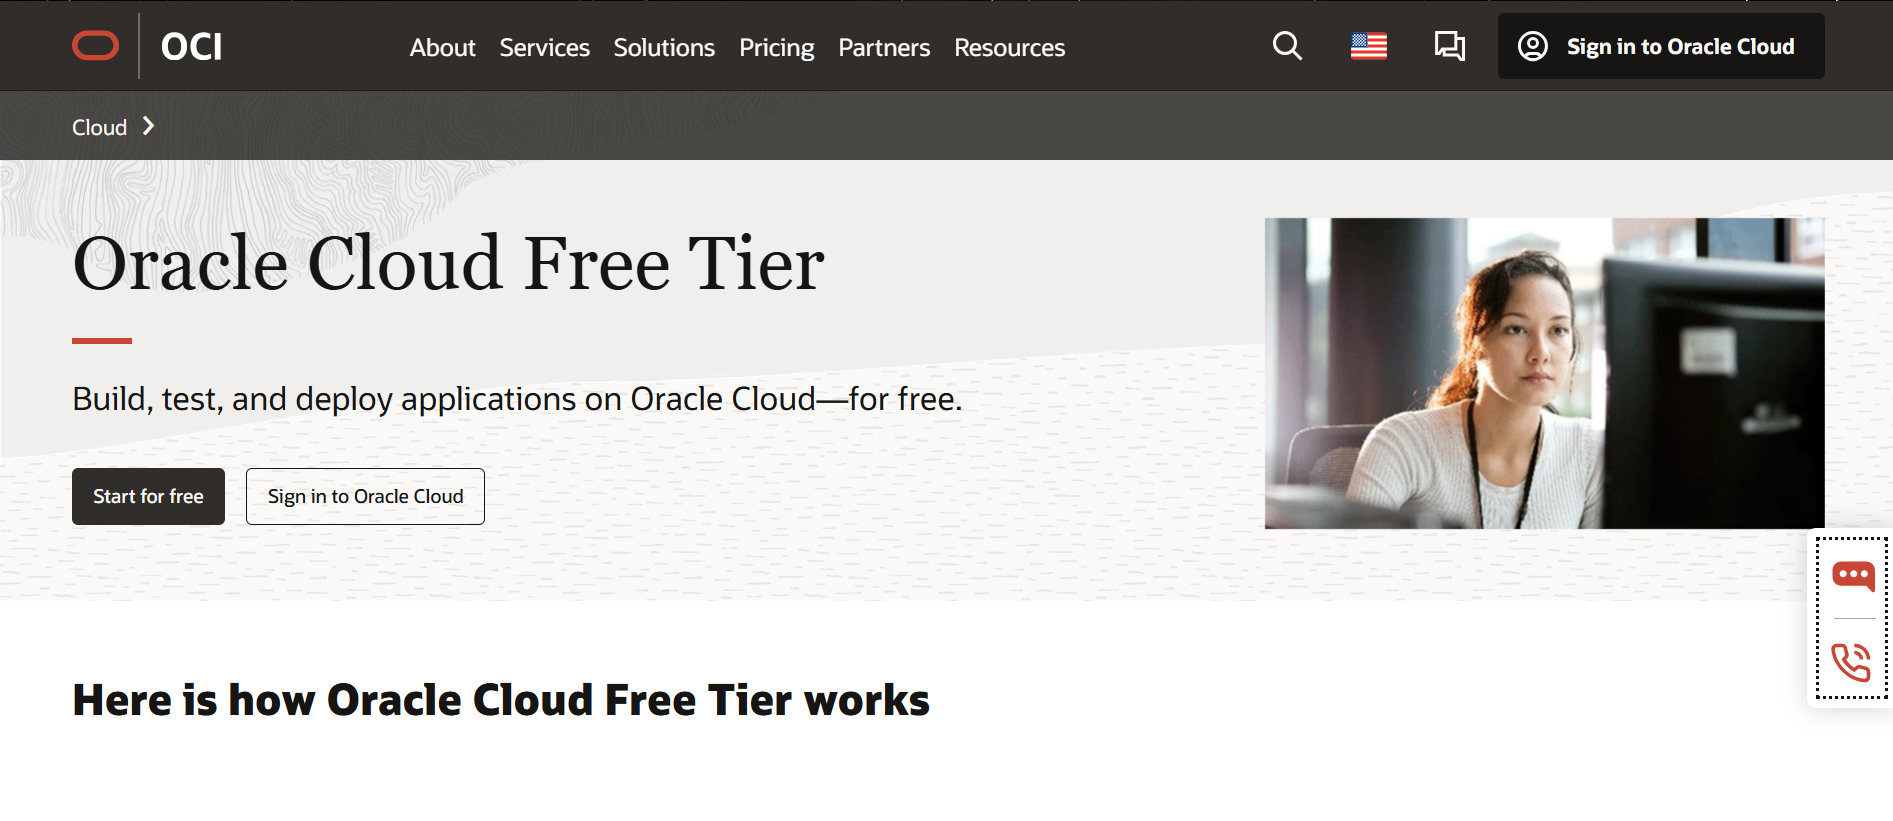
\includegraphics[width=0.7\textwidth]{Demo/Giao_dien_truy_cap.png}
    \caption{Giao diện khi truy cập vào trang web OCI}
    \label{fig:cloud_intro}
\end{figure}

\item Bước 2: Điền thông tin cơ bản của người dùng và nhấn Verity my email để tiếp tục.

\begin{figure}[H] % cần gói float nếu muốn fix vị trí
    \centering
    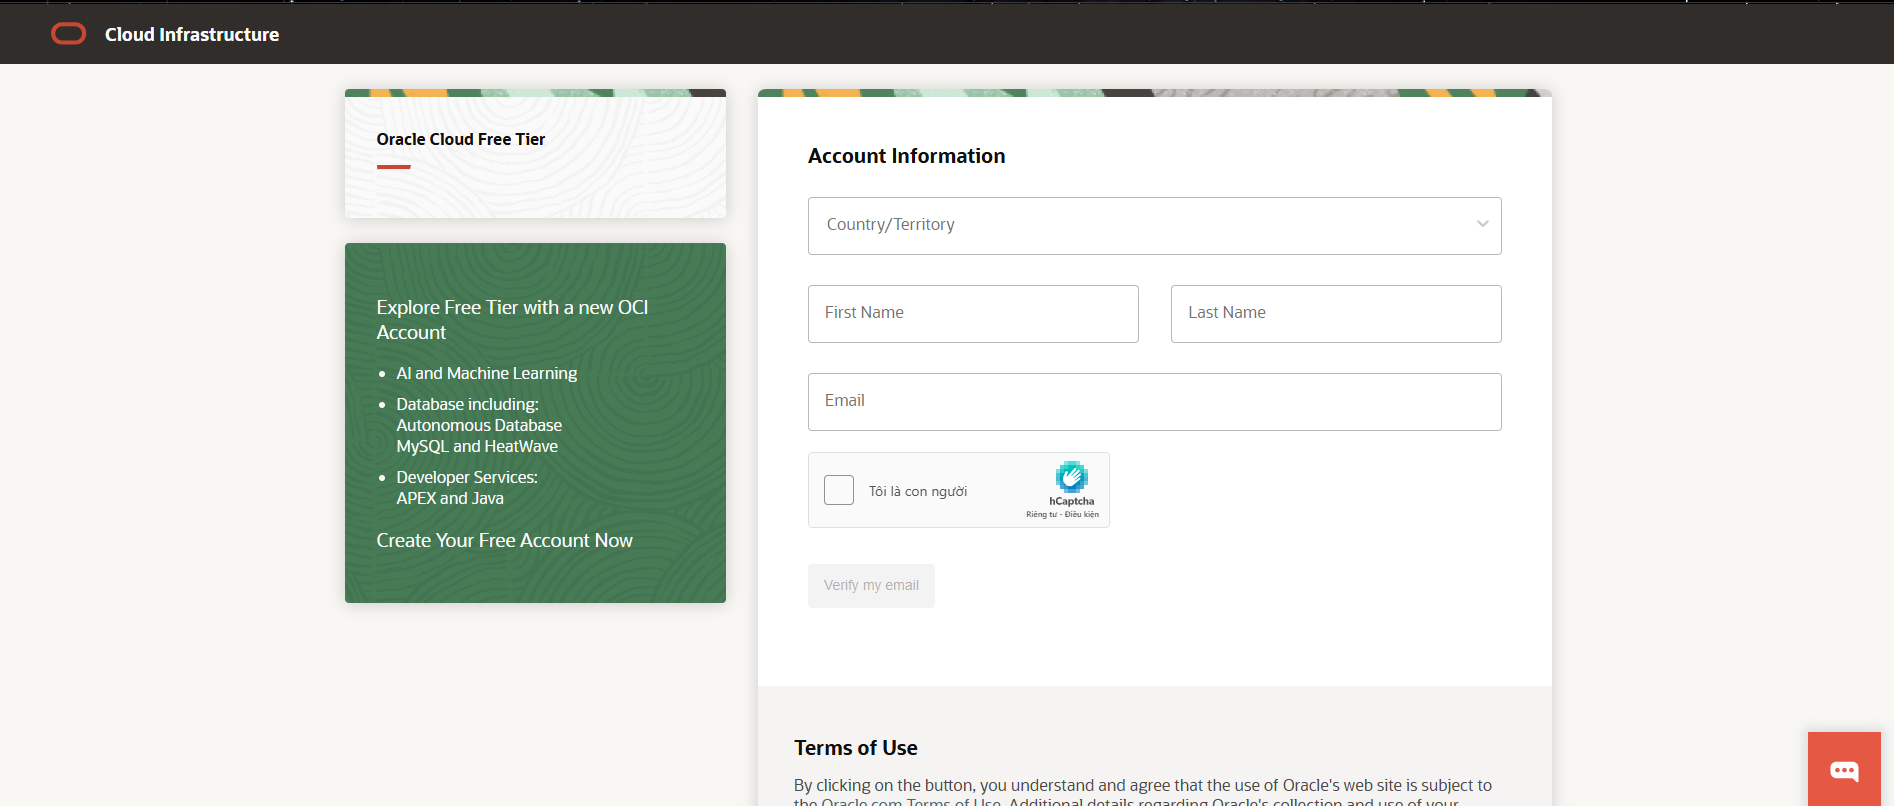
\includegraphics[width=0.9\textwidth]{Demo/Account_Information.png}
    \caption{Giao diện Account Information điền thông tin cơ bản}
    \label{fig:cloud_intro}
\end{figure}

\item Bước 3: Điền các thông tin về tài khoản đăng nhập vào các ô để tiếp tục.

\begin{figure}[H] % cần gói float nếu muốn fix vị trí
    \centering
    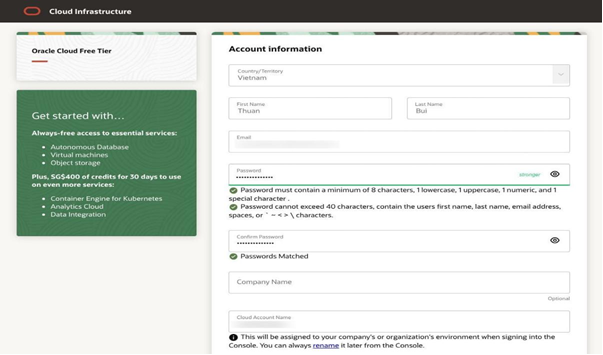
\includegraphics[width=0.9\textwidth]{Demo/Account_Information_dang_nhap.png}
    \caption{Giao diện Account Information điền các thông tin đăng nhập}
    \label{fig:cloud_intro}
\end{figure}

\item Bước 4: Nhập thông tin cá nhân: Địa chỉ (Address),Điện thoại (Phone Number) và Payment verification.

\begin{figure}[H] % cần gói float nếu muốn fix vị trí
    \centering
    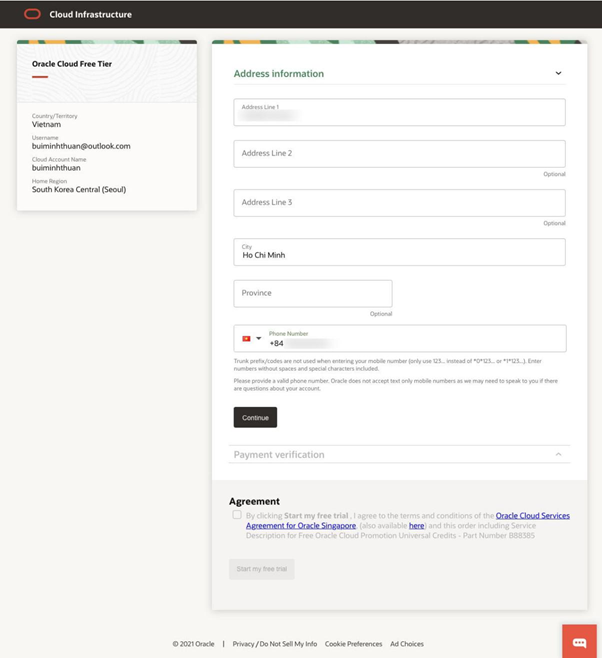
\includegraphics[width=0.7\textwidth]{Demo/Address_Information.png}
    \caption{Giao diện Address Information}
    \label{fig:cloud_intro}
\end{figure}

\item Bước 5: Bấm Continue, đợi hệ thống xử lý và hoàn tất quá trình tạo tài khoản.

\begin{figure}[H] % cần gói float nếu muốn fix vị trí
    \centering
    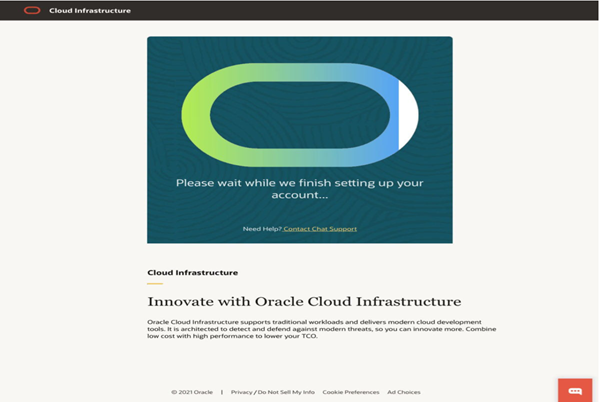
\includegraphics[width=0.7\textwidth]{Demo/Cho_doi_hoan_tat.png}
    \caption{Giao diện chờ đợi quá trình hoàn tất tạo tài khoản.}
    \label{fig:cloud_intro}
\end{figure}

\end{myitem}

\subsubsection{Đăng nhập}
\begin{myitem}
\item Bước 1: Tiến hành truy cập theo vào trang https://www.oracle.com/cloud/sign-in.html và nhập điền tên tài khoản đăng nhập vào Cloud Account Name.

\begin{figure}[H] % cần gói float nếu muốn fix vị trí
    \centering
    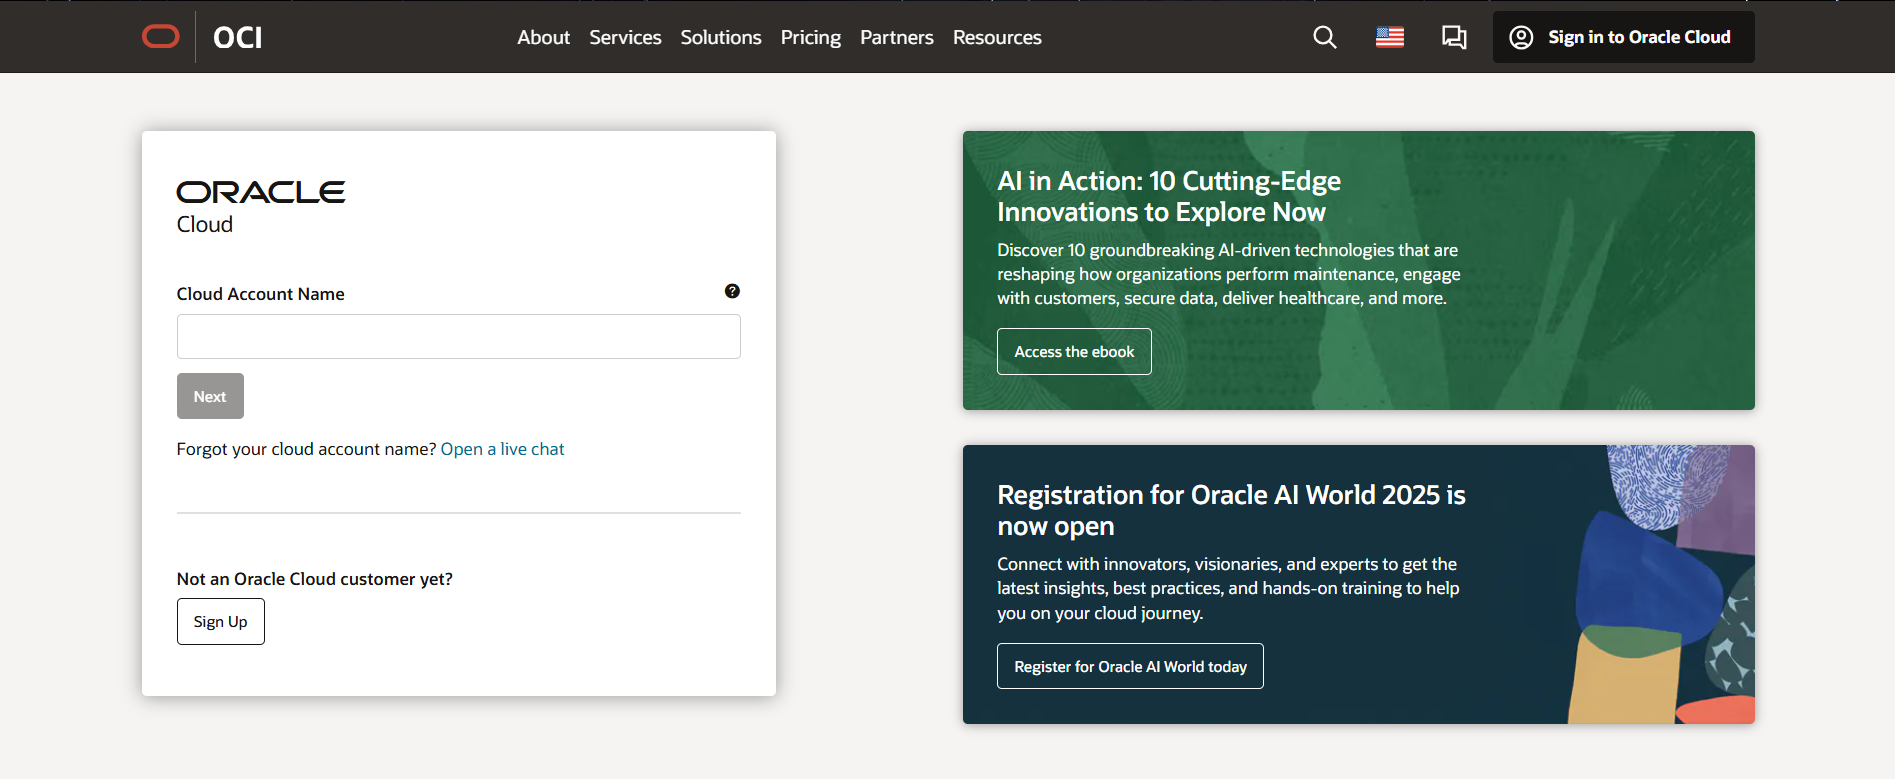
\includegraphics[width=0.9\textwidth]{Demo/Trang_dang_nhap.png}
    \caption{Giao diện trang đăng nhập tài khoản}
    \label{fig:cloud_intro}
\end{figure}

\item Bước 2: Nhập tiếp email của chúng ta vào ô User Name và mật khẩu vào ô Password.

\begin{figure}[H] % cần gói float nếu muốn fix vị trí
    \centering
    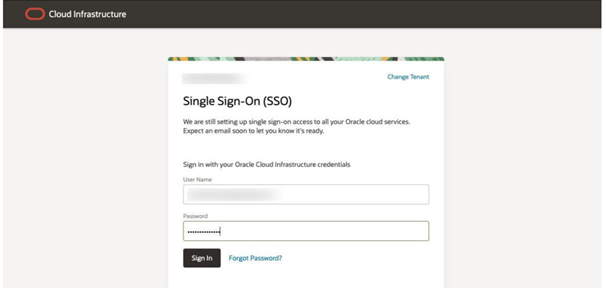
\includegraphics[width=0.9\textwidth]{Demo/Single_Sign_On.png}
    \caption{Giao diện Single Sign-On (SSO)}
    \label{fig:cloud_intro}
\end{figure}

\item Bước 3: Nhấn Sign In, đăng nhập thành công vào Dashboard của Oracle Cloud.

\begin{figure}[H] % cần gói float nếu muốn fix vị trí
    \centering
    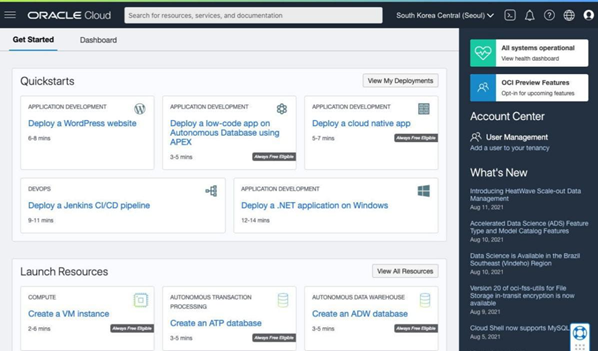
\includegraphics[width=0.9\textwidth]{Demo/Dang_nhap_thanh_cong.png}
    \caption{Giao diện đăng nhập thành công vào Dashboard của Oracle Cloud}
    \label{fig:cloud_intro}
\end{figure}

\end{myitem}

\subsection{Các dịch vụ của Oracle cloud}
\subsubsection{Cơ sở hạ tầng như một dịch vụ (IaaS)}
Oracle Cloud Infrastructure (OCI) cung cấp mô hình dịch vụ hạ tầng như một dịch vụ (IaaS) với khả năng tính toán mạnh mẽ, linh hoạt và đáp ứng được nhiều loại hình công việc khác nhau. Các dịch vụ tính toán trải dài từ máy chủ vật lý (bare metal) cho những nhu cầu xử lý trực tiếp và toàn quyền kiểm soát phần cứng, đến máy ảo (VM) phù hợp với các ứng dụng cần khả năng mở rộng nhanh chóng, tiết kiệm chi phí. Bên cạnh đó, OCI còn hỗ trợ bộ xử lý đồ họa (GPU) dành cho các tác vụ chuyên sâu như trí tuệ nhân tạo (AI), học máy (ML), xử lý dữ liệu lớn (Big Data) và phân tích hình ảnh. Đối với những yêu cầu đặc thù về tính toán hiệu suất cao (HPC), OCI cung cấp các cấu hình tối ưu hóa để xử lý các mô phỏng khoa học, phân tích kỹ thuật và khối lượng công việc yêu cầu tốc độ xử lý cực lớn. Ngoài ra, nền tảng cũng hỗ trợ điều phối vùng chứa (Container orchestration), giúp triển khai và quản lý các ứng dụng container hóa trên quy mô lớn với độ ổn định cao.

Về lưu trữ, OCI mang đến nhiều tùy chọn linh hoạt phù hợp với từng nhu cầu sử dụng: lưu trữ cục bộ cho các tác vụ cần tốc độ truy xuất nhanh, lưu trữ khối (Block Storage) để phục vụ cơ sở dữ liệu và các ứng dụng quan trọng, lưu trữ tệp (File Storage) cho môi trường cần chia sẻ dữ liệu qua nhiều hệ thống, cũng như lưu trữ đối tượng (Object Storage) cho các dữ liệu phi cấu trúc, sao lưu, lưu trữ lâu dài hoặc phân phối nội dung. Ngoài ra, còn có lưu trữ lưu trữ kho (Archive Storage) dành cho khối lượng công việc lớn nhưng ít truy cập, giúp tối ưu chi phí trong khi vẫn đảm bảo khả năng truy xuất khi cần.

Một trong những đặc điểm nổi bật của OCI là thiết kế hạ tầng mạng với trọng tâm bảo mật và độc lập cao. Khả năng ảo hóa mạng của OCI được xây dựng tách rời khỏi lớp điều khiển của người giám sát (hypervisor). Điều này giúp giảm thiểu rủi ro bảo mật thường gặp trong các hệ thống ảo hóa truyền thống, hạn chế khả năng tấn công vào lớp hypervisor, đồng thời cung cấp cho khách hàng một môi trường mạng ảo hóa an toàn, tin cậy hơn. Người dùng có thể dễ dàng tạo và quản lý mạng đám mây ảo (VCN), tùy chỉnh các cấu hình mạng như phân đoạn, tường lửa, cổng kết nối và VPN, đảm bảo khả năng tích hợp linh hoạt với hệ thống tại chỗ (on-premises).

Nhờ những yếu tố trên, IaaS của OCI không chỉ mang đến hạ tầng mạnh mẽ, an toàn mà còn giúp doanh nghiệp tối ưu hiệu suất, giảm chi phí vận hành, tăng khả năng mở rộng và sẵn sàng đáp ứng mọi yêu cầu từ những ứng dụng phổ thông đến các hệ thống phức tạp, khối lượng công việc quan trọng.

\subsubsection{Nền tảng như một dịch vụ (PaaS)}
Nền tảng như một dịch vụ (PaaS) của Oracle Cloud Infrastructure được xây dựng dựa trên hạ tầng IaaS, kết hợp sức mạnh của các công nghệ Oracle với nhiều khuôn khổ mã nguồn mở hiện đại. PaaS cung cấp cho doanh nghiệp một môi trường phát triển toàn diện, giúp đơn giản hóa việc xây dựng, triển khai và quản lý các ứng dụng, cơ sở dữ liệu cũng như các quy trình kinh doanh. Một số nhóm dịch vụ PaaS nổi bật của OCI gồm:

\begin{myitem}
    \item Phát triển ứng dụng: Cung cấp cho các nhà phát triển công cụ để thiết kế, viết mã, kiểm thử và triển khai các ứng dụng thông minh, hiện đại trực tiếp trên nền tảng đám mây, rút ngắn thời gian phát triển và tăng khả năng mở rộng.
    
    \item Cơ sở dữ liệu đám mây: Cho phép tổ chức truy cập các phiên bản hiệu suất cao của Oracle Autonomous Database, nhờ đó giảm bớt gánh nặng quản trị, tối ưu hóa hiệu suất và nâng cao tính bảo mật của dữ liệu.
    Quản lý nội dung: Hỗ trợ doanh nghiệp xây dựng và quản lý nội dung số trên một nền tảng tập trung, giúp nhanh chóng cá nhân hóa trải nghiệm khách hàng, đồng thời đảm bảo tính nhất quán trong quản lý dữ liệu và tài nguyên số.
    Tích hợp ứng dụng và dữ liệu: Cung cấp các công cụ để kết nối và tích hợp nhiều ứng dụng, hệ thống và nguồn dữ liệu khác nhau, từ đó hình thành các quy trình làm việc mượt mà và tạo điều kiện cho phân tích chuyên sâu.

    \item Phân tích kinh doanh (Business Analytics): Cho phép doanh nghiệp khai thác tối đa giá trị dữ liệu nhờ các giải pháp phân tích mạnh mẽ, kết hợp với thuật toán machine learning tích hợp sẵn, nhằm đưa ra thông tin toàn diện (BI) phục vụ quyết định chiến lược.
    
\end{myitem}

Nhờ hệ sinh thái PaaS toàn diện này, OCI mang đến cho các tổ chức khả năng đẩy nhanh đổi mới, giảm chi phí quản lý, nâng cao hiệu suất làm việc và khai thác dữ liệu hiệu quả hơn.

\subsubsection{Phần mềm như một dịch vụ (SaaS)}
Các dịch vụ SaaS của Oracle Cloud Infrastructure (OCI) cung cấp những ứng dụng được triển khai sẵn và luôn sẵn sàng để sử dụng, giúp doanh nghiệp dễ dàng áp dụng vào nhiều tình huống thực tế. Thông qua SaaS, các tổ chức có thể nhanh chóng tự động hóa nhiều hoạt động quan trọng như quản lý nguồn nhân lực (HRM), lập kế hoạch nguồn lực doanh nghiệp (ERP), bán hàng và tiếp thị, quản lý chuỗi cung ứng (SCM) cũng như quản lý tài chính. Với mô hình này, doanh nghiệp không cần lo lắng về việc cài đặt, bảo trì hay cập nhật phần mềm mà vẫn có thể tận dụng các giải pháp hiện đại để nâng cao hiệu quả vận hành và tối ưu quy trình kinh doanh.

\subsubsection{Dữ liệu như một dịch vụ (DaaS)}
Dữ liệu như một dịch vụ (DaaS) của Oracle Cloud Infrastructure là một nền tảng tổng hợp và phân phối dữ liệu, cho phép doanh nghiệp khai thác thông tin một cách hiệu quả, chính xác và kịp thời. Với OCI DaaS, người dùng có thể truy cập vào kho dữ liệu khổng lồ gồm hơn 135 triệu bản ghi liên hệ toàn cầu, đi kèm hơn 90 thuộc tính doanh nghiệp (firmographics) khác nhau, từ quy mô tổ chức, lĩnh vực hoạt động, doanh thu cho đến vị trí địa lý.

Không chỉ cung cấp dữ liệu, DaaS còn hỗ trợ chuẩn hóa và làm sạch dữ liệu liên hệ theo thời gian thực, giúp loại bỏ trùng lặp, sửa lỗi và đảm bảo tính chính xác của thông tin. Điều này đặc biệt hữu ích trong các hoạt động tiếp thị, bán hàng, phân tích khách hàng và ra quyết định chiến lược, nơi dữ liệu đáng tin cậy đóng vai trò cốt lõi.

Bên cạnh đó, OCI DaaS mang đến cho doanh nghiệp khả năng truy cập dữ liệu theo cách hoàn chỉnh, cập nhật liên tục và phù hợp với từng nhu cầu cụ thể, giúp nâng cao chất lượng phân tích, tối ưu hóa quy trình kinh doanh và hỗ trợ mạnh mẽ cho các sáng kiến chuyển đổi số.

\subsection{Đánh giá về An toàn bảo mật}
Oracle Cloud là một trong những nền tảng đám mây phổ biến và mạnh mẽ hiện nay, với các tính năng bảo mật và an toàn được thiết kế chặt chẽ. Dưới đây là một số điểm nổi bật về an toàn và bảo mật của Oracle Cloud:

\subsubsection{Bảo mật dữ liệu và mã hóa}
\begin{myitem}
    
\item Mã hóa toàn diện
\begin{mysubitem}
    \item Oracle Cloud triển khai cơ chế mã hóa dữ liệu toàn diện, bao gồm cả quá trình truyền tải dữ liệu (in transit) và khi dữ liệu đang được lưu trữ (at rest). Điều này có nghĩa là dù dữ liệu đang di chuyển giữa người dùng và hệ thống, hay đã được lưu giữ trong các máy chủ và dịch vụ lưu trữ của Oracle, nó đều được bảo vệ bởi các thuật toán mã hóa hiện đại. Cách tiếp cận này giúp đảm bảo dữ liệu không thể bị khai thác trái phép trong suốt vòng đời của nó, ngay cả khi bị chặn ở giữa đường truyền.

    \item Ngoài ra, việc áp dụng mã hóa ở nhiều lớp khác nhau trong Oracle Cloud còn giúp giảm thiểu rủi ro trước các mối đe dọa bảo mật ngày càng tinh vi. Người dùng có thể yên tâm rằng mọi thông tin nhạy cảm như dữ liệu khách hàng, tài chính hay thông tin kinh doanh quan trọng đều được che chắn, khiến kẻ tấn công gần như không thể sử dụng dữ liệu ngay cả khi có được quyền truy cập vật lý hoặc logic.
\end{mysubitem}


\item Quản lý khóa
\begin{mysubitem}
    \item Một trong những ưu điểm nổi bật của Oracle Cloud là hệ thống quản lý khóa (Key Management) mạnh mẽ và linh hoạt. Oracle cho phép khách hàng sử dụng các khóa mã hóa riêng của mình thay vì phụ thuộc hoàn toàn vào nhà cung cấp dịch vụ. Cách tiếp cận này không chỉ tăng tính chủ động mà còn giúp doanh nghiệp đáp ứng tốt hơn các yêu cầu tuân thủ pháp lý và quy định về bảo mật dữ liệu.

    \item Hệ thống quản lý khóa của Oracle được thiết kế với khả năng kiểm soát chi tiết, từ việc tạo, phân phối, lưu trữ đến việc xoay vòng và thu hồi khóa. Nhờ đó, người dùng có thể dễ dàng thiết lập chính sách bảo mật phù hợp với nhu cầu riêng của tổ chức. Đồng thời, giải pháp này cũng hạn chế rủi ro mất mát hoặc lạm dụng khóa, vốn có thể gây ảnh hưởng nghiêm trọng đến tính an toàn của dữ liệu.
\end{mysubitem}

\item Mã hóa phía máy chủ
\begin{mysubitem}
    \item Oracle Cloud triển khai cơ chế mã hóa mạnh mẽ ngay từ phía máy chủ để bảo vệ dữ liệu trong cơ sở dữ liệu và các dịch vụ lưu trữ. Điều này có nghĩa là dữ liệu sẽ được tự động mã hóa khi được ghi vào hệ thống lưu trữ, mà không đòi hỏi sự can thiệp phức tạp từ phía người dùng. Với cách tiếp cận này, Oracle đảm bảo tính đơn giản trong quá trình sử dụng, đồng thời vẫn duy trì mức độ bảo mật cao cho toàn bộ dữ liệu.

    \item Việc mã hóa phía máy chủ còn giúp tăng cường khả năng bảo vệ dữ liệu trong nhiều tình huống khác nhau, bao gồm cả các trường hợp kẻ tấn công có thể truy cập trực tiếp vào cơ sở hạ tầng vật lý. Bằng việc sử dụng các thuật toán mã hóa chuẩn quốc tế và cơ chế bảo mật nhiều lớp, Oracle Cloud tạo ra một môi trường an toàn, giúp doanh nghiệp yên tâm lưu trữ và xử lý những thông tin quan trọng nhất của mình.

\end{mysubitem}

\end{myitem}

\subsubsection{Quản lý quyền truy cập}
\begin{myitem}
    \item Identity and Access Management (IAM):
    \begin{mysubitem}
        \item Trong Oracle Cloud, hệ thống Identity and Access Management (IAM) đóng vai trò trung tâm trong việc bảo vệ tài nguyên và dữ liệu. Thay vì để tất cả người dùng có quyền ngang nhau, IAM cho phép quản trị viên xác định chính xác ai có quyền truy cập, họ có thể thực hiện những hành động gì, và trên tài nguyên nào. Điều này giúp tổ chức tránh được rủi ro từ việc lạm dụng quyền hoặc truy cập trái phép, đồng thời tạo ra một môi trường quản lý minh bạch và an toàn hơn. IAM còn hỗ trợ việc phân chia trách nhiệm, giúp các bộ phận trong tổ chức chỉ được cấp quyền phù hợp với công việc của mình, không dư thừa, cũng không thiếu sót.

        \item Ngoài ra, IAM trên Oracle Cloud được thiết kế linh hoạt, có thể mở rộng cùng với sự phát triển của doanh nghiệp. Khi quy mô tổ chức thay đổi, quản trị viên chỉ cần chỉnh sửa hoặc tạo thêm các vai trò (roles) và chính sách (policies) để điều chỉnh quyền truy cập. Điều này giúp giảm bớt công sức quản lý thủ công, đồng thời đảm bảo rằng ngay cả khi tổ chức phát triển nhanh chóng, hệ thống quyền truy cập vẫn được kiểm soát chặt chẽ và thống nhất. IAM cũng hỗ trợ cơ chế ghi nhật ký (audit log), nhờ đó doanh nghiệp có thể theo dõi lịch sử truy cập, phát hiện kịp thời những hành vi bất thường hoặc nghi ngờ có dấu hiệu tấn công.
    \end{mysubitem}

    \item Chính sách xác thực:
    \begin{mysubitem}
        \item Để tăng cường mức độ an toàn, Oracle Cloud không chỉ dừng lại ở việc phân quyền mà còn áp dụng nhiều chính sách xác thực khác nhau. Một trong những phương pháp phổ biến và quan trọng là xác thực đa yếu tố (Multi-Factor Authentication – MFA). Với MFA, người dùng không thể đăng nhập chỉ bằng mật khẩu thông thường, mà cần thêm một yếu tố khác như mã xác thực từ ứng dụng di động, tin nhắn SMS hoặc thiết bị bảo mật chuyên dụng. Cơ chế này giúp giảm thiểu rủi ro khi mật khẩu bị rò rỉ hoặc tấn công bởi hacker, bởi vì kẻ xấu vẫn không thể truy cập nếu thiếu yếu tố xác thực bổ sung.

        \item Bên cạnh MFA, Oracle Cloud cũng hỗ trợ tích hợp với các hệ thống nhận diện người dùng sẵn có của doanh nghiệp, ví dụ như Active Directory hay các dịch vụ nhận dạng khác. Điều này mang lại sự tiện lợi vì người dùng không cần phải tạo thêm tài khoản mới, mà có thể dùng chính tài khoản doanh nghiệp của mình để truy cập dịch vụ đám mây. Nhờ vậy, tổ chức vừa đơn giản hóa việc quản lý danh tính, vừa đảm bảo đồng bộ hóa dữ liệu và quy trình bảo mật giữa hệ thống nội bộ và nền tảng đám mây. Cách tiếp cận này đặc biệt hữu ích với các doanh nghiệp lớn, nơi có số lượng nhân viên đông đảo và nhu cầu phân quyền phức tạp.
    \end{mysubitem}
    
\end{myitem}

\subsubsection{Kiểm soát và giám sát}
\begin{myitem}
    \item Oracle Cloud Guard:
    \begin{mysubitem}
        \item Trong một hệ thống đám mây phức tạp, việc giám sát liên tục là vô cùng quan trọng để phát hiện sớm những dấu hiệu bất thường. Oracle Cloud Guard được thiết kế để thực hiện chính xác nhiệm vụ này. Công cụ này liên tục quan sát các hoạt động trong môi trường đám mây, tự động phát hiện những hành vi không tuân thủ chính sách bảo mật hoặc có khả năng gây rủi ro. Ví dụ, Cloud Guard có thể nhận diện khi một người dùng cố gắng truy cập vào tài nguyên mà họ không được phép, khi một cấu hình dịch vụ bị thay đổi trái phép, hoặc khi có sự xuất hiện của lưu lượng bất thường có thể là dấu hiệu của một cuộc tấn công mạng. Nhờ khả năng phát hiện kịp thời, tổ chức có thể ngăn chặn và xử lý sớm các mối đe dọa, giảm thiểu thiệt hại.

        \item Bên cạnh đó, Oracle Cloud Guard không chỉ dừng lại ở việc giám sát và cảnh báo, mà còn cung cấp khả năng tự động phản ứng với sự cố. Quản trị viên có thể cấu hình các hành động phản hồi tự động, chẳng hạn như vô hiệu hóa một tài khoản đáng ngờ, chặn lưu lượng truy cập từ địa chỉ IP rủi ro, hoặc khôi phục cấu hình dịch vụ về trạng thái an toàn trước đó. Điều này giúp doanh nghiệp không chỉ giám sát thụ động mà còn chủ động ứng phó, tăng tốc quá trình bảo mật. Với Cloud Guard, tổ chức có trong tay một công cụ mạnh mẽ giúp duy trì an toàn, đảm bảo rằng môi trường đám mây luôn được kiểm soát chặt chẽ.
    \end{mysubitem}

    \item Audit and Logging:
    \begin{mysubitem}
        \item Để duy trì một hệ thống an toàn, việc theo dõi và ghi lại toàn bộ hoạt động của người dùng cũng như các dịch vụ trong đám mây là yếu tố then chốt. Oracle Cloud cung cấp các tính năng Audit và Logging, cho phép hệ thống tự động ghi nhận mọi hành động, từ những thao tác quản trị như tạo, sửa, hoặc xóa tài nguyên, đến những giao dịch hàng ngày của ứng dụng và người dùng. Các bản ghi này đóng vai trò như “nhật ký hoạt động” chi tiết, giúp doanh nghiệp có cái nhìn toàn diện về những gì đang diễn ra trong hệ thống. Nhờ đó, khi xảy ra sự cố, quản trị viên có thể dễ dàng truy vết, xác định nguyên nhân, và biết rõ ai là người thực hiện hành động nào, vào thời điểm nào.

        \item Ngoài vai trò trong điều tra sự cố, Audit và Logging còn hỗ trợ mạnh mẽ cho công tác tuân thủ các quy định về bảo mật và pháp lý. Nhiều tổ chức hoạt động trong các lĩnh vực đặc thù như tài chính, y tế hay chính phủ thường phải đáp ứng những tiêu chuẩn khắt khe về quản lý dữ liệu. Việc có đầy đủ nhật ký và báo cáo kiểm tra từ Oracle Cloud giúp doanh nghiệp dễ dàng chứng minh rằng họ đã thực hiện các biện pháp bảo mật theo đúng yêu cầu. Bên cạnh đó, dữ liệu ghi nhật ký cũng có thể được tích hợp với các hệ thống phân tích hoặc SIEM (Security Information and Event Management) để phát hiện sớm các mẫu hành vi bất thường, từ đó tăng cường khả năng phòng ngừa tấn công trong tương lai.
    \end{mysubitem}
    
\end{myitem}

\subsubsection{Các biện pháp phòng ngừa tấn công}
\begin{myitem}
    \item Dịch vụ bảo mật chủ động:
    \begin{mysubitem}
        \item Trong môi trường điện toán đám mây, các cuộc tấn công từ bên ngoài luôn là mối đe dọa thường trực đối với hệ thống và dữ liệu. Để đối phó với những nguy cơ này, Oracle cung cấp một loạt dịch vụ bảo mật chủ động, trong đó quan trọng nhất là tường lửa (firewall) và cơ chế bảo vệ trước các cuộc tấn công từ chối dịch vụ phân tán (DDoS). Tường lửa đóng vai trò như một “lá chắn” đầu tiên, kiểm soát mọi luồng dữ liệu ra vào hệ thống, chỉ cho phép những kết nối hợp lệ và ngăn chặn các yêu cầu truy cập trái phép. Song song với đó, dịch vụ bảo vệ DDoS của Oracle giúp giảm thiểu rủi ro từ các cuộc tấn công với mục tiêu làm nghẽn tài nguyên, đảm bảo hệ thống vẫn duy trì hoạt động ổn định ngay cả khi bị kẻ xấu cố tình tạo ra lưu lượng truy cập giả mạo quá tải.

        \item Không chỉ dừng lại ở mức phòng thủ, các dịch vụ bảo mật chủ động còn hỗ trợ cơ chế giám sát theo thời gian thực, cho phép phát hiện và phản ứng nhanh với các mối đe dọa. Nhờ hệ thống được cập nhật liên tục về các mẫu tấn công mới nhất, Oracle có khả năng ngăn chặn ngay cả những kỹ thuật xâm nhập tinh vi mà hacker thường sử dụng. Điều này giúp doanh nghiệp giảm thiểu thiệt hại và tăng cường khả năng duy trì dịch vụ mà không bị gián đoạn. Với các giải pháp bảo mật đa lớp này, Oracle Cloud mang đến một môi trường vận hành an toàn, ổn định và đáng tin cậy hơn cho người dùng.
    \end{mysubitem}

    \item Quản lý các điểm yếu bảo mật:
    \begin{mysubitem}
        \item Một trong những nguyên nhân phổ biến khiến hệ thống dễ bị tấn công là sự tồn tại của các lỗ hổng phần mềm và cấu hình sai. Nhằm giải quyết vấn đề này, Oracle cung cấp các công cụ chuyên dụng để phát hiện, phân tích và khắc phục kịp thời các điểm yếu bảo mật trong hệ thống. Các công cụ này có thể quét tự động trên toàn bộ môi trường đám mây để tìm ra những lỗ hổng tiềm ẩn, đồng thời phân loại mức độ nguy hiểm của chúng. Nhờ vậy, quản trị viên có thể dễ dàng xác định đâu là vấn đề cần ưu tiên xử lý trước, tránh việc bỏ sót hoặc xử lý sai thứ tự ưu tiên.

        \item Bên cạnh việc phát hiện, hệ thống còn hỗ trợ các giải pháp khắc phục tự động hoặc gợi ý biện pháp xử lý phù hợp. Điều này giúp doanh nghiệp giảm thiểu thời gian tồn tại của lỗ hổng, ngăn chặn kẻ tấn công lợi dụng để xâm nhập. Ngoài ra, Oracle cũng cung cấp các bản vá và cập nhật bảo mật thường xuyên, đảm bảo rằng phần mềm và hạ tầng luôn ở trạng thái an toàn nhất. Với cách tiếp cận chủ động và toàn diện, quản lý điểm yếu bảo mật không chỉ là biện pháp khắc phục mà còn trở thành một phần quan trọng trong chiến lược phòng ngừa, giúp nâng cao khả năng chống chịu trước các mối đe dọa ngày càng tinh vi.
    \end{mysubitem}
    
\end{myitem}

\subsection{Ưu điểm - nhược điểm của Oracle cloud}
\subsubsection{Ưu điểm}

\begin{myitem}
    \item Khả năng xây dựng dựa trên các giải pháp on-premise sẵn có: Các doanh nghiệp đã đầu tư nhiều vào các giải pháp on-premise có thể chuyển chúng sang cloud một cách dễ dàng với toàn quyền kiểm soát, ví dụ: ảo hóa, thiết lập máy chủ và lưu trữ cũng như vị trí trung tâm dữ liệu, đồng thời doanh nghiệp có thể tùy chọn sử dụng kiến thức chuyên môn của Oracle khi cần \cite{gimasys_oci_benefits}.

    \item Tăng hiệu suất: Các doanh nghiệp dù đang ở quy mô nào cũng cần những ứng dụng liên tục được cập nhập. Cơ sở hạ tầng đám mây Oracle cung cấp các máy chủ đơn giản có thể xử lý các tập dữ liệu khổng lồ theo thời gian thực, tận dụng cơ sở dữ liệu Oracle có hiệu suất cao, có khả năng mở rộng cao và các công nghệ liên quan như Oracle Real Applications Clusters. Các máy chủ này cũng sử dụng bộ nhớ nhanh (NVME) với khả năng xử lý vài chục terabyte theo mỗi trường hợp \cite{gimasys_oci_benefits}.

    \item Tính bảo mật cao: Doanh nghiệp cần các ứng dụng, mạng và dữ liệu với tính bảo mật cao nhằm tránh những vi phạm có thể xảy ra ảnh hưởng đến danh tiếng của mình. Cơ sở hạ tầng đám mây Oracle được xây dựng chú trọng đặc biệt vào khả năng bảo mật:

    \begin{mysubitem}
        \item Tách biệt giữa tài nguyên mạng và điện toán

        \item Cho phép thiết lập khả năng bảo vệ chuyên sâu thông qua tường lửa tích hợp 
        
        \item Tích hợp với các công cụ quản lý truy cập danh tính

        \item Xác thực đa yếu tố 
        
        \item Mã hóa dữ liệu.

    \end{mysubitem}

    \item Kiến trúc mở : Với Cơ sở hạ tầng đám mây Oracle, doanh nghiệp sẽ không bắt buộc phải sử dụng giải pháp của một nhà cung cấp duy nhất. Doanh nghiệp có thể chạy khối lượng công việc trên Oracle hoặc trên nền tảng khác, nhưng vẫn giữ được khả năng tương tác thông qua việc tuân thủ các tiêu chuẩn. Thêm vào đó, OCI hỗ trợ công nghệ open-source và tạo ngôn ngữ lập trình với khả năng tích hợp DevOps và các công cụ công nghệ thông tin từ các nhà cung cấp khác nhau và chạy trên cả máy chủ Windows và Linux \cite{gimasys_oci_benefits}.
\end{myitem}

\subsubsection{Nhược điểm}
\begin{myitem}
    \item Chi phí cao đối với doanh nghiệp nhỏ: Mặc dù Oracle cung cấp một số mô hình chi phí linh hoạt, nhưng về tổng thể, chi phí sử dụng Oracle Cloud có thể cao hơn so với các đối thủ như AWS hay Google Cloud, đặc biệt đối với các doanh nghiệp nhỏ hoặc các dự án có quy mô nhỏ. Điều này có thể là một yếu tố cản trở đối với những doanh nghiệp có ngân sách hạn chế.

    \item Hệ sinh thái không rộng như các đối thủ lớn: Mặc dù Oracle Cloud cung cấp nhiều dịch vụ đám mây mạnh mẽ, nhưng so với AWS và Azure, hệ sinh thái của Oracle Cloud có thể chưa rộng và đa dạng bằng. Các công cụ và dịch vụ bổ sung (third-party services) và số lượng các đối tác hỗ trợ cũng không nhiều như đối thủ.
    
    \item Hạn chế về hỗ trợ khu vực: Mạng lưới trung tâm dữ liệu: Dù Oracle Cloud đang mở rộng nhanh chóng, nhưng vẫn còn hạn chế về số lượng trung tâm dữ liệu trên toàn cầu so với AWS hoặc Azure. Điều này có thể làm hạn chế khả năng tối ưu hóa độ trễ và khả năng phục hồi trong một số khu vực địa lý.

\end{myitem}

\subsection{Thử nghiệm dịch vụ OCI Language Service}
\subsubsection{Giới thiệu về dịch vụ}
Trong mục này, chúng ta giới thiệu cách thiết lập Oracle Cloud Infrastructure (OCI) Python SDK và cách bắt đầu với OCI Language Service. Bằng việc triển khai thử nghiệm, chúng ta đóng gói mã nguồn vào một lớp (class) để thuận tiện cho việc kiểm thử nhanh chóng các chức năng của dịch vụ \cite{medium_exploring_oci_language_service}.

Việc thực hiện thử nghiệm này không chỉ giúp chúng ta nắm rõ quy trình cài đặt và sử dụng, mà còn tạo tiền đề để khai thác sâu hơn các tính năng phân tích ngôn ngữ mà OCI Language Service cung cấp.

\begin{figure}[H] % cần gói float nếu muốn fix vị trí
    \centering
    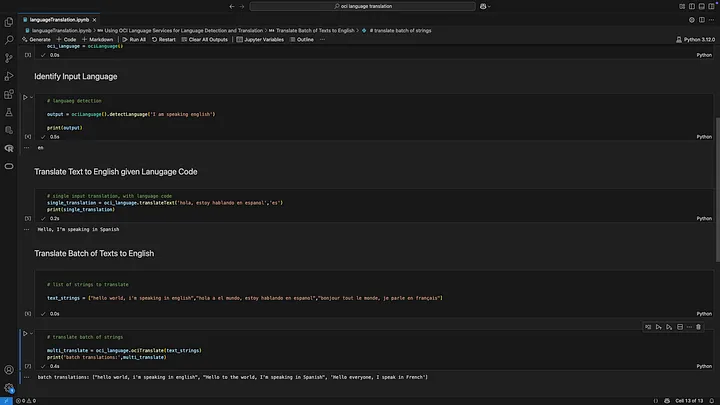
\includegraphics[width=0.9\textwidth]{Demo/Dich_nhieu_chuoi_van_ban.jpg}
    \caption{Thực hiện dịch nhiều chuỗi văn bản thông qua một lớp tùy chỉnh}
    \label{fig:cloud_intro}
\end{figure}

OCI Language Service là một dịch vụ API dễ sử dụng, cung cấp các mô hình ngôn ngữ đã được huấn luyện sẵn trên nền tảng OCI \cite{medium_exploring_oci_language_service}.

Sử dụng OCI Language Service, chúng ta có thể thực hiện các tác vụ sau:

\begin{myitem}
    \item Phát hiện ngôn ngữ (Language Detection)

    \item Phân loại văn bản (Text Classification)
    
    \item Phân tích cảm xúc (Sentiment Analysis)
    
    \item Trích xuất cụm từ khóa (Key Phrase Extraction)
    
    \item Nhận diện thực thể có tên (NER) (Named Entity Recognition)
    
    \item Phát hiện thông tin cá nhân (PII Detection)
    
    \item Xử lý ngôn ngữ tự nhiên trong lĩnh vực y tế (Healthcare NLP)
\end{myitem}

Dịch vụ này cũng cho phép chúng ta huấn luyện các mô hình tùy chỉnh để phân loại và nhận diện thực thể trên các bộ dữ liệu riêng của mình.

\subsubsection{Bắt đầu với OCI Python SDK}
OCI SDK cho Python cho phép chúng ta viết mã để quản lý các tài nguyên trên OCI cũng như gọi các dịch vụ đám mây như GenAI, Language, Vision, v.v.

Khi chạy mã trên máy tính cá nhân, chúng ta có thể dễ dàng thiết lập API key trong OCI Console, từ đó bắt đầu tương tác với các tài nguyên OCI thông qua SDK hoặc OCI CLI.

Để thiết lập API key, chúng ta thực hiện các bước sau:
\begin{myitem}
    \item Truy cập OCI Console.

    \item Vào mục My Profile trong Identity \& Security.
    
    \item Chọn Add API Key để thêm khóa API mới.
\end{myitem}

\begin{figure}[H] % cần gói float nếu muốn cố định vị trí
    \centering
    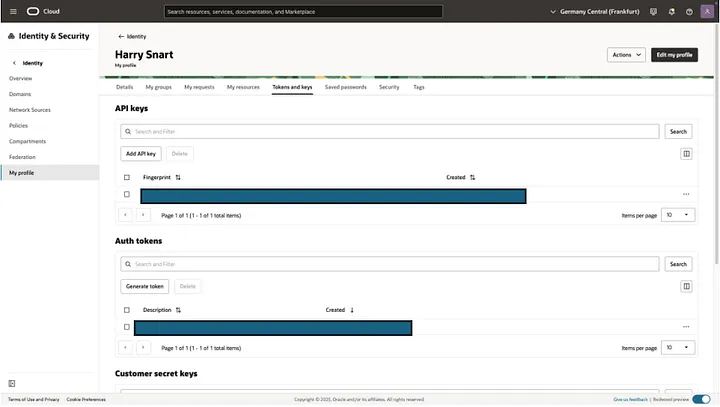
\includegraphics[width=0.9\textwidth, keepaspectratio]{Demo/Them_API_key (1).jpg}
    \caption{Thêm một API Key mới vào hồ sơ OCI}
    \label{fig:cloud_intro}
\end{figure}

Sau đó, hệ thống sẽ hỏi chúng ta muốn tạo mới hay tải lên một cặp khóa (key pair). Khi các khóa đã được tải xuống, chúng ta có thể thêm API Key mới vào hồ sơ OCI của mình.

\begin{figure}[H] % cần gói float nếu muốn cố định vị trí
    \centering
    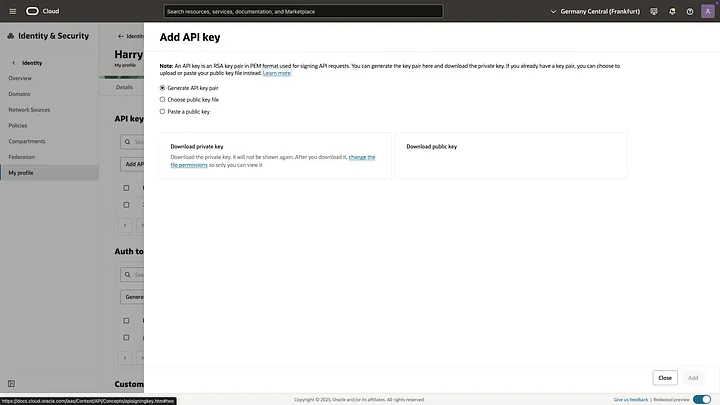
\includegraphics[width=0.9\textwidth, keepaspectratio]{Demo/Chon_cap_khoa.jpg}
    \caption{Chọn cặp khóa (key pair) cho API Key}
    \label{fig:cloud_intro}
\end{figure}

Hệ thống sẽ cung cấp cho chúng ta một mã nhận dạng duy nhất và tự động tạo một hồ sơ (profile).

\begin{figure}[H] % cần gói float nếu muốn cố định vị trí
    \centering
    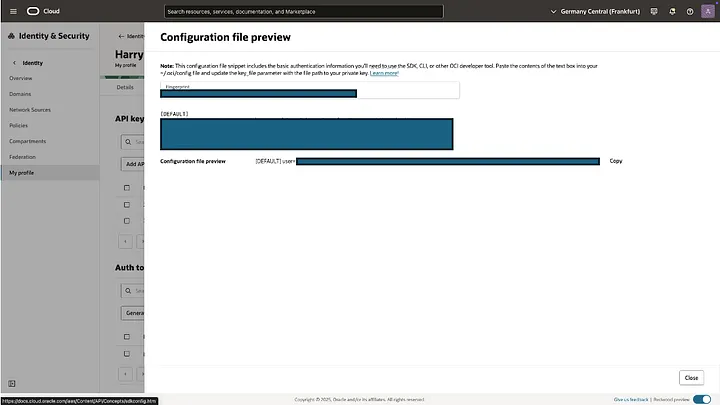
\includegraphics[width=0.95\textwidth, keepaspectratio]{Demo/Cau_hinh.jpg}
    \caption{Tạo tệp cấu hình cho API Key}
    \label{fig:cloud_intro}
\end{figure}

Theo mặc định, OCI SDK sẽ tìm tệp cấu hình tại:

\begin{center}
\fbox{\parbox{0.8\textwidth}{\texttt{~/.oci/config}}}
\end{center}

\textit{Lưu ý: nếu chúng ta có nhiều tenancy hoặc nhiều profile, chúng ta có thể thiết lập nhiều profile trong tệp cấu hình — chỉ cần đảm bảo không kết nối với profile DEFAULT khi sử dụng SDK.}

\subsubsection{Phát hiện ngôn ngữ (Language Detection)}
Chúng ta sẽ bắt đầu với API Phát hiện ngôn ngữ (Language Detection API). Dịch vụ này cho phép xử lý nhiều yêu cầu cùng lúc (batch), hỗ trợ phát hiện lên đến 100 bản ghi mỗi lần gọi API. API có thể nhận diện hơn 100 ngôn ngữ khác nhau.

Điều quan trọng cần lưu ý là mỗi lần gọi API chỉ trả về một ngôn ngữ chính. Nếu chúng ta gửi một batch chứa nhiều tài liệu đa ngôn ngữ, API sẽ trả về ngôn ngữ chiếm ưu thế trong batch đó.

Với OCI Python SDK, chúng ta có thể sử dụng các hàm trợ giúp (helper functions) để tạo payload đúng định dạng cho API theo phong cách Python, giúp việc gọi API trở nên thuận tiện và trực quan \cite{medium_exploring_oci_language_service}.

\begin{lstlisting}
# load python sdk for OCI
import oci

# instantiate an AI Client using config from profile
ai_client = oci.ai_language.AIServiceLanguageClient(oci.config.from_file())

# create function to detect input language
def detectLanguage(ai_client,text):
    ''' Detect language of input string, returning code '''
    doc1 = oci.ai_language.models.DominantLanguageDocument(key='key1', text=text)
    documents = [doc1]
    batch_detect_dominant_language_details = oci.ai_language.models.BatchDetectDominantLanguageDetails(documents=documents)
    output = ai_client.batch_detect_dominant_language(batch_detect_dominant_language_details)
    return output.data.documents[0].languages[0].code

# run function
detectLanguage("Hello world, I'm speaking English")

\end{lstlisting}

\subsubsection{Dịch ngôn ngữ (Language Translation)}
Để sử dụng API Dịch ngôn ngữ (Translation API), chúng ta có thể dùng SDK theo cách tương tự: chúng ta khởi tạo một client, sau đó sử dụng phương thức batch\_language\_translation.

Phương thức này cho phép chúng ta:
\begin{myitem}
    \item Đặt ngôn ngữ đầu vào cho từng tài liệu trong batch.

    \item Chọn ngôn ngữ đích mà chúng ta muốn dịch sang.

\end{myitem}

chúng ta có thể thực hiện dịch thời gian thực (real-time translation) hoặc dịch bất đồng bộ (asynchronous translation) cho các tệp lớn khi cần xử lý hàng loạt.

\begin{lstlisting}
# load python sdk for OCI
import oci

# instantiate an AI Client using config from profile
ai_client = oci.ai_language.AIServiceLanguageClient(oci.config.from_file())

# create function to translate text given language code    
def translateToEnglish(ai_client, input_text, language_code):
    ''' Translate text to English if not already English '''
    text_document =  oci.ai_language.models.TextDocument(
         key="1",
         text=input_text,
         language_code=language_code)
    
    try:
        # Run text classification on text_document
        text_translation = ai_client.batch_language_translation(
            batch_language_translation_details=oci.ai_language.models.BatchLanguageTranslationDetails(
                documents=[text_document],
                target_language_code="en"
            )
        )
        # return the data
        return text_translation.data.documents[0].translated_text


    # Print any API errors
    except Exception as e:
        print(e)
    return

# run function with sample string
translateToEnglish(ai_client,'hola, estoy hablando en espanol','es')

\end{lstlisting}

\subsubsection{Dịch đa ngôn ngữ theo batch (Batch Multi-Lingual Translation)}
Đối với dịch thời gian thực (real-time translation), việc kết hợp dịch vụ Phát hiện ngôn ngữ (Language Detection) và dịch vụ Dịch ngôn ngữ (Translation) khá đơn giản, cho phép tạo ra các bản dịch từ nhiều ngôn ngữ đầu vào khác nhau.

Ví dụ, đoạn code dưới đây có thể hữu ích như một bước tiền xử lý (pre-processing) cho Retrieval Augmented Generation (RAG) trên bộ sưu tập tài liệu đa ngôn ngữ, trước khi tiến hành chia nhỏ (chunking) và tách tài liệu.

\begin{lstlisting}
final_strings = []

for sentence in text_strings:
    language_code = detectLanguage(ai_client,sentence)
    
    if language_code != 'en':
        try:
            sentence = translateToEnglish(ai_client,sentence, language_code)
        except:
            print('language not supported!')
            sentence = 'language not supported for:'+sentence
    final_strings.append(sentence)

print('translated texts:', final_strings)

\end{lstlisting}

Cách làm này giúp chúng ta tạo ra bộ sưu tập tài liệu thống nhất về một ngôn ngữ, từ đó có thể sử dụng các mô hình embedding nhỏ hơn và hiệu quả hơn.

Để thuận tiện cho việc trình bày, đây là đoạn code gói gọn thành một lớp Python (Python class) nhằm minh họa cách các dịch vụ có thể hoạt động phối hợp với nhau.

\begin{lstlisting}
# load custom class
from ociLanguage import ociLanguage

# define OCI language client
oci_language = ociLanguage()

# list of strings to translate
text_strings = ["hello world, i'm speaking in english","hola a el mundo, estoy hablando en espanol","bonjour tout le monde, je parle en français"]

# translate batch of strings
multi_translate = oci_language.ociTranslate(text_strings)
print('batch translations:',multi_translate)

\end{lstlisting}

\newpage
\subsection*{\centering KẾT LUẬN CHƯƠNG 3}
\addcontentsline{toc}{subsection}{KẾT LUẬN CHƯƠNG 3}

Chương 3 đã cung cấp một cái nhìn tổng quan và chi tiết về dịch vụ điện toán đám mây của Oracle Cloud Infrastructure (OCI), từ việc tìm hiểu các loại dịch vụ chính (IaaS, PaaS, SaaS, DaaS) đến các quy trình đăng ký, đăng nhập và thử nghiệm thực tế với OCI Language Service. Qua các phân tích và thí nghiệm, có thể rút ra một số nhận định quan trọng như sau:

Trước hết, OCI nổi bật với hiệu năng cao, khả năng mở rộng linh hoạt và tính bảo mật vượt trội. Các tính năng như Autonomous Database, quản lý khóa và mã hóa dữ liệu, cùng với hệ thống IAM và Cloud Guard, đảm bảo dữ liệu của doanh nghiệp luôn được bảo vệ toàn diện. Đồng thời, cơ chế tự động hóa và hỗ trợ API giúp giảm thiểu khối lượng công việc vận hành, từ đó nâng cao hiệu quả triển khai và quản lý tài nguyên trên nền tảng đám mây.

Thứ hai, các dịch vụ thử nghiệm như OCI Language Service cho thấy khả năng ứng dụng thực tiễn của nền tảng trong lĩnh vực trí tuệ nhân tạo và xử lý ngôn ngữ tự nhiên. Việc tích hợp phát hiện ngôn ngữ, dịch thuật đa ngôn ngữ, phân loại văn bản và trích xuất thực thể cho thấy OCI không chỉ phục vụ nhu cầu hạ tầng mà còn cung cấp các giải pháp thông minh, hỗ trợ doanh nghiệp trong các nhiệm vụ phân tích dữ liệu và tự động hóa quy trình nghiệp vụ.

Bên cạnh các ưu điểm, chúng ta cũng nhận thấy một số hạn chế của Oracle Cloud, như chi phí tương đối cao đối với doanh nghiệp nhỏ, hệ sinh thái dịch vụ chưa rộng bằng các đối thủ lớn, và hạn chế về phạm vi trung tâm dữ liệu. Tuy nhiên, những nhược điểm này vẫn có thể được cân nhắc và quản lý thông qua lựa chọn gói dịch vụ phù hợp và tối ưu hóa quy trình triển khai.

\newpage

\plainsection{KẾT LUẬN}
Qua quá trình nghiên cứu và thực hành, có thể khẳng định rằng Oracle Cloud Infrastructure (OCI) là một nền tảng điện toán đám mây toàn diện, mang lại nhiều lợi ích cho doanh nghiệp và tổ chức. OCI cung cấp các dịch vụ đa dạng, từ hạ tầng ảo hóa, cơ sở dữ liệu, đến các dịch vụ trí tuệ nhân tạo, giúp triển khai ứng dụng, quản lý dữ liệu và tối ưu hóa quy trình một cách hiệu quả. Hạ tầng mạnh mẽ, khả năng mở rộng linh hoạt cùng hiệu năng cao là những điểm nổi bật, đáp ứng nhu cầu về tính sẵn sàng, bảo mật và hiệu quả hoạt động.

Quá trình thực hành và triển khai các dịch vụ trên OCI cho thấy nền tảng này không chỉ mạnh về hạ tầng mà còn thân thiện với người dùng. Việc quản lý tài nguyên, cấu hình mạng, triển khai máy chủ và sử dụng các công cụ giám sát, bảo mật giúp đảm bảo an toàn dữ liệu, giảm thiểu rủi ro và tăng cường kiểm soát cho tổ chức. Điều này minh chứng rằng OCI là một môi trường đáng tin cậy, hỗ trợ các doanh nghiệp khai thác tối đa tiềm năng công nghệ đám mây.

Đặc biệt, các dịch vụ thông minh của OCI, như OCI Language Service, mở ra khả năng phân tích ngôn ngữ, nhận diện thực thể và phân tích cảm xúc, hỗ trợ đa ngôn ngữ và xử lý dữ liệu một cách thông minh. Những tính năng này chứng tỏ Oracle Cloud không chỉ là nền tảng hạ tầng mà còn là công cụ phát triển ứng dụng thông minh, phù hợp với xu hướng chuyển đổi số và trí tuệ nhân tạo hiện nay.

Tổng kết lại, mặc dù vẫn còn một số hạn chế về chi phí và mạng lưới trung tâm dữ liệu, nhưng OCI với những ưu điểm về hiệu suất, bảo mật, tính mở rộng và khả năng ứng dụng thông minh vẫn là lựa chọn tối ưu cho các tổ chức muốn triển khai giải pháp đám mây hiện đại, an toàn và hiệu quả. Tiểu luận này đã cung cấp cái nhìn toàn diện, từ lý thuyết đến thực hành và ứng dụng, giúp nâng cao hiểu biết và khả năng khai thác các dịch vụ đám mây của Oracle.

\newpage

\clearpage
\Urlmuskip=0mu plus 2mu\relax
\def\UrlBreaks{\do\/\do-\do\.\do\_\do\?\do\&\do\#}

% --- loại bỏ mọi tiêu đề mặc định của thư mục tài liệu ---
\makeatletter
\renewcommand{\refname}{}   % cho article
% xóa câu lệnh tạo \section* hoặc \chapter* trong môi trường thebibliography
\patchcmd{\thebibliography}{\section*{\refname}}{}{}{}
\patchcmd{\thebibliography}{\chapter*{\bibname}}{}{}{}
\makeatletter

% ====== tiêu đề tài liệu tham khảo (tự viết) ======
% ====== tiêu đề tài liệu tham khảo ======
\plainsection{TÀI LIỆU THAM KHẢO}
\addcontentsline{toc}{section}{TÀI LIỆU THAM KHẢO}

% Làm lỏng dãn cách để tránh tràn lề với chuỗi dài (URL)
\begingroup
\sloppy
\bibliographystyle{IEEEtran}
\bibliography{references}
\endgroup
\newpage

\end{maincontent}

\end{document}
